\documentclass[]{article}
\usepackage[utf8]{inputenc}
\usepackage[top=3cm, bottom=3cm, left=2cm, right=2cm]{geometry}

\usepackage{amsmath}
\usepackage{graphicx}
\graphicspath{{img/}}
\usepackage{wrapfig}
\usepackage{braket}
\usepackage{multicol}

\title{Scintillating Counter of Uranium and Thorium (SCOUT)}
\author{Morgan Askins}
\date{Updated: \today}

\begin{document}
\maketitle
\begin{center}    
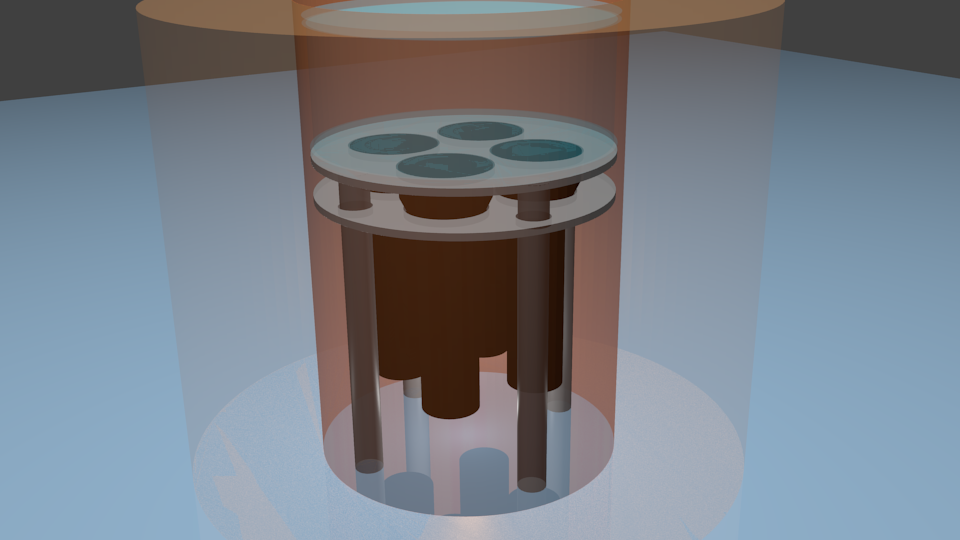
\includegraphics[width=0.8\linewidth]{scout_render.png}
\end{center}
\section{Introduction}
\begin{wrapfigure}{r}{0.25\textwidth}
  \centering
  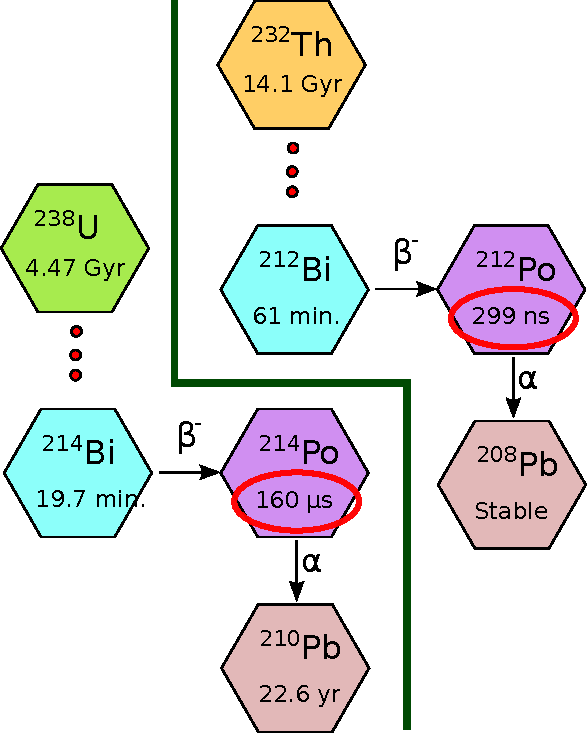
\includegraphics[width=0.25\textwidth]{DecayChain.pdf}
\end{wrapfigure}
Scout is an alpha beta coincidence counter designed to assess the radiopurity of the SNO+
liquid scintillator (Linear Alkylbenzene + 2 g/L 2,5 diphenyloxazole) that arrives
at the surface transfer facility at Snolab. By counting the decays of 
$^{214}Bi\rightarrow^{214}Po\rightarrow^{210}Pb$ in the Uranium decay chain and 
$^{212}Bi\rightarrow^{212}Po\rightarrow^{208}Pb$ in the Thorium decay chain, the
radiopurity can be determined. The expected sensitivity for each of these is of
order $10^{-10}$ g/g for a 24 hour measurement.

\section{Design}
The design for Scout consists of a lead shield from a previous Germanium counter at
UCDavis roughly 4.5" thick. The shield is copper lined on the inside. The inner vessel
is made of acrylic which is
coupled to the PMTs. The vessel holds roughly 5 liters of fluid in a short, but wide
cylindrical volume.
Room is left at the bottom for high voltage and signal cables to run from the voltage
dividers out the hole in the bottom of the shield to the DAQ. Room is left at the top to
accommodate quick-connect ports for gas and liquid exchange at the top.
\begin{center}
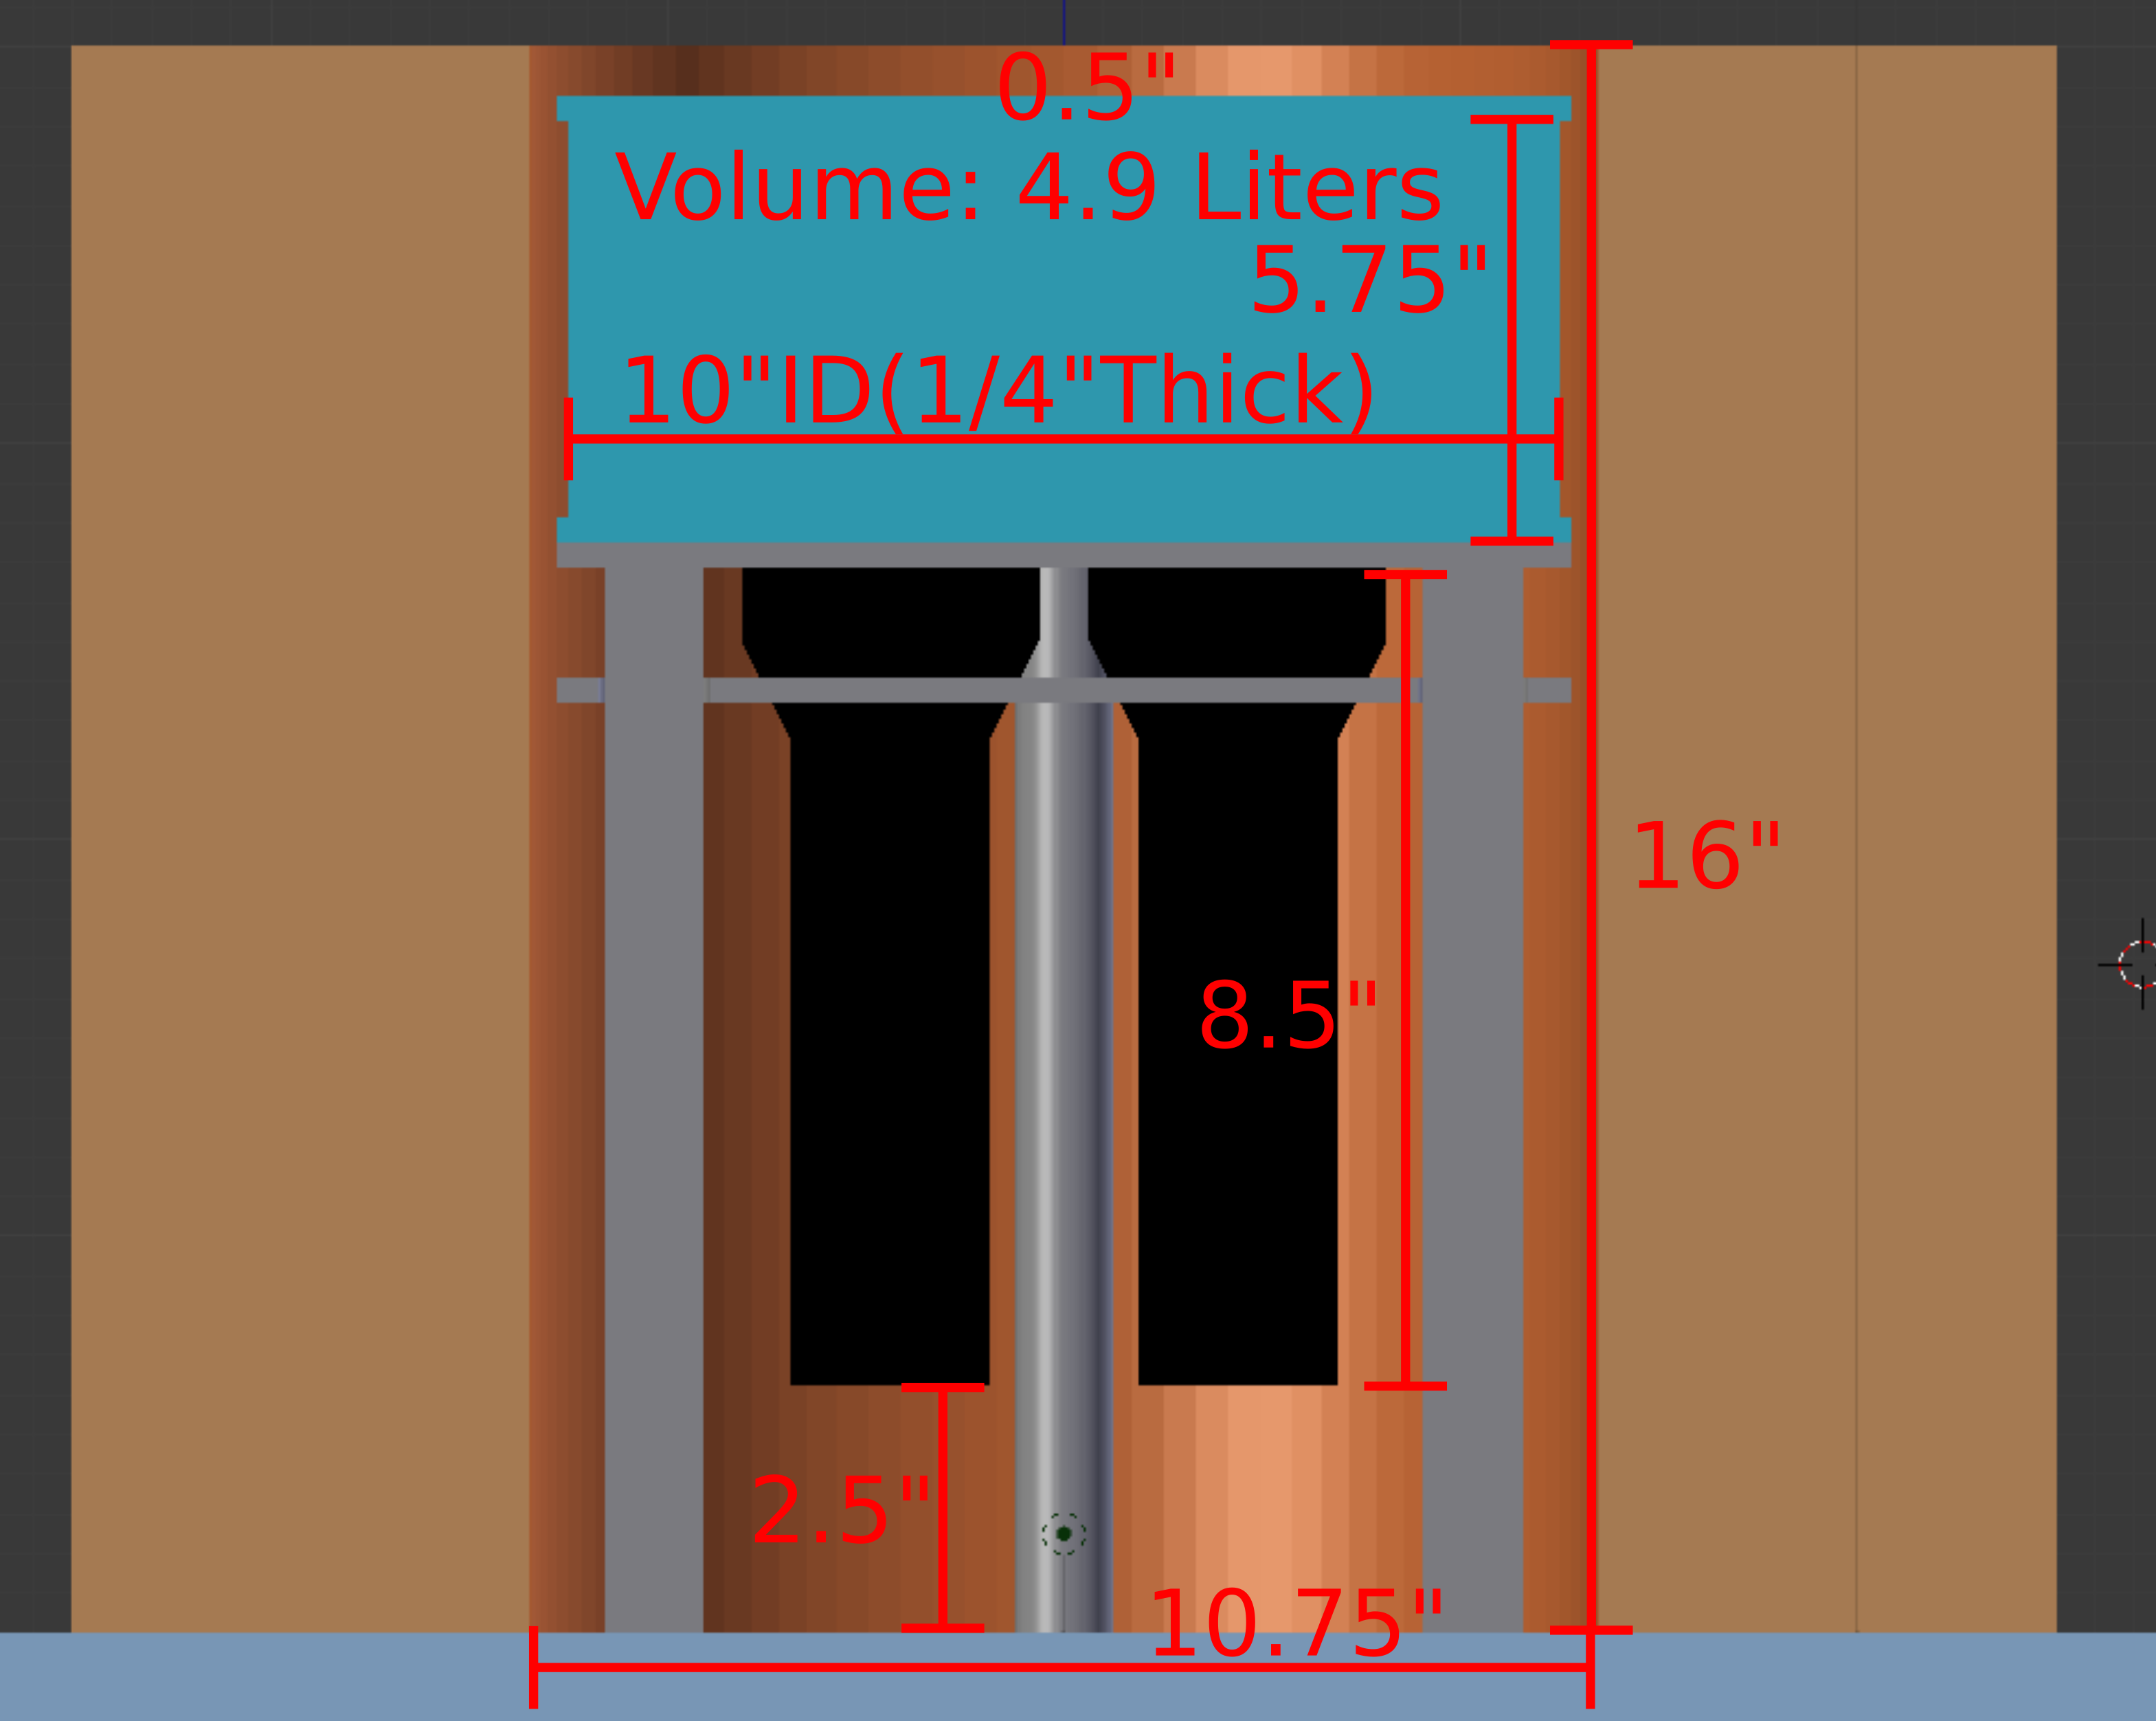
\includegraphics[width=0.5\textwidth]{flat_scout.png}
\end{center}

\section{Data Acquisition}
The four photomultipliers are powered by a desktop CAEN high voltage power supply. The supply
has four channels, so the voltage can be individually adjusted for proper gain matching. The
voltage dividers are negative with a BNC and SHV connector coming directly from them. The BNC
will convert to LIMO and plug into the 16-channel SIS3316 250MHz ADC where only four channels
will be used. The trigger scheme in software can either be set to sum the four channels or
trigger on individual channels. There is not currently a way to require two channels to go
above threshold, but this may be looked into in the future. The coincidence trigger will be
done offline using timing and energy cuts.

\section{Sensitivity}
With the assumption that the LAB is clean to begin with, limtis will be set based on the background
rates, detector volume, and live time. The coincidence window for Bi-Po will help to reject most single
events except those that fall in the same random coincidence window. Based on the energy resolution
of the final design, an energy cut can help to further reduce the background event rate. For a detector
volume of about 5 liters, the sensitivity for a 1 hour run would be about $10^{-10}$ g/g for each
isotope, with $^{238}$U having a slightly better result due to the shorter half-life.

\section{Procedure}
\begin{enumerate}
  \item Assuming we use 5 liters of LAB, measure out PPO at 2g/L (10 grams total) into the
    mixing vessel.
  \item Seal the mixing vessel and connect the nitrogen supply line to the vessel.
  \item Set the pressure on the nitrogen supply to about 0.5 to 1 psi. A check valve
    located at the top of the vessel will open at 0.5 psi purging the vessel. Allow the
    purging to continue for about 1 minute.
  \item Turn off and disconnect the nitrogen supply.
  \item Fill the mixing vessel with 5 liters of LAB, keeping track of the mass of LAB
    added on a scale. This will be the primary means of knowing the sensitive volume in Scout.
  \item Gently swirl the mixture to make sure the PPO dissolves into the LAB. It is likely
    that the PPO will already be mixed in due to the turbulence from adding the LAB.
  \item Seal the acrylic vessel and connect the nitrogen supply line and purge just like the
    mixing vessel. The acrylic vessel has the same connections and check valve that the mixing
    vessel does.
  \item Turn off and disconnect the nitrogen supply. This time keep both hoses attached to the
    acrylic vessel and filled with nitrogen.
  \item Quick-connect the hoses to the mixing vessel, using one for fluid transfer and the
    other to allow free gas exchange between the two.
  \item Tilt the vessel in such a way that fluid flows freely through the fluid port,
    and gas flows freely through the gas port. A small portion of the scintillator will be
    left in the mixing vessel which can be discarded at the end.
  \item Weigh the mass of the mixing vessel once more to determine the mass transfered into
    the acrylic vessel.
  \item Disconnect the fluid and gas lines from the acrylic vessel, close the top of the lead
    shield, and wrap the shield in a black tarp (just in case of small light leaks).
  \item Begin data acquisition (procedure to be written).
  \item Once all data has been acquired the top of the acrylic vessel can be taken off for 
    draining and cleaning.
  \item Using a hand pump start a siphon from the acrylic vessel into the 55-gallon waste
    drum.
  \item Clean up any remaining LAB in the vessel with an absorbant cloth and dispose of
    properly.
  \item {[}It may be possible to clean the AV by filling and rinsing with UPW or clean LAB{]}
\end{enumerate}

\section{Component List}
\begin{itemize}
  \item 1 metric tonne lead shield on Stand: 2'x2'x5' tall
  \item Waste drum (55 Gallon)
  \item Acrylic Measurement Vessel (~ 5 liters)
  \item Mobile mixing vessel
  \item Fluid transfer hose with hand valves on both ends
  \item Gas transfer hose with hand valves on both ends
  \item 4x3" Photomultipliers
  \item Desktop High Voltage Supply (Caen)
  \item VME Crate
  \item VME Waveform Digitizer (sis3316 ADC)
  \item Intel NUC for data recording
  \item External backup storage
  %\item Magnetic Stirrer
  \item Chemical Spill Kit
  \item Tubing to connect
\end{itemize}

%\begin{wrapfigure}{r}{0.25\textwidth}
%  \centering
%  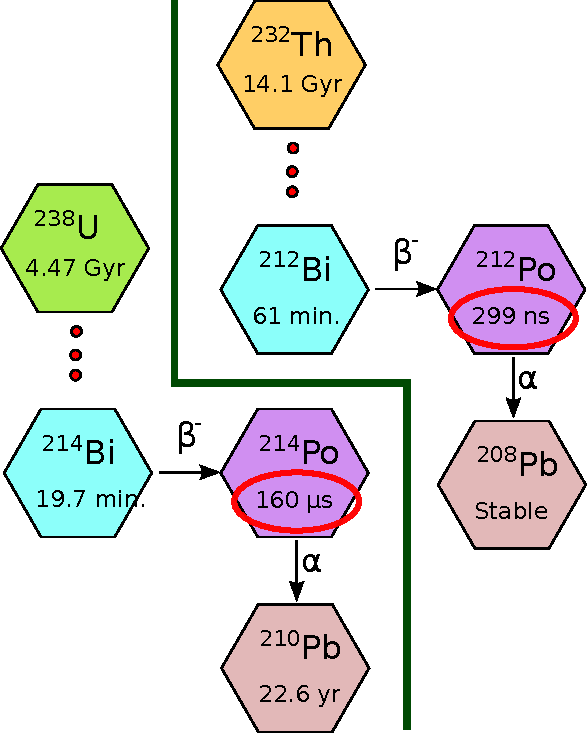
\includegraphics[width=0.25\textwidth]{DecayChain.pdf}
%\end{wrapfigure}

\section{Images}
\begin{figure}
  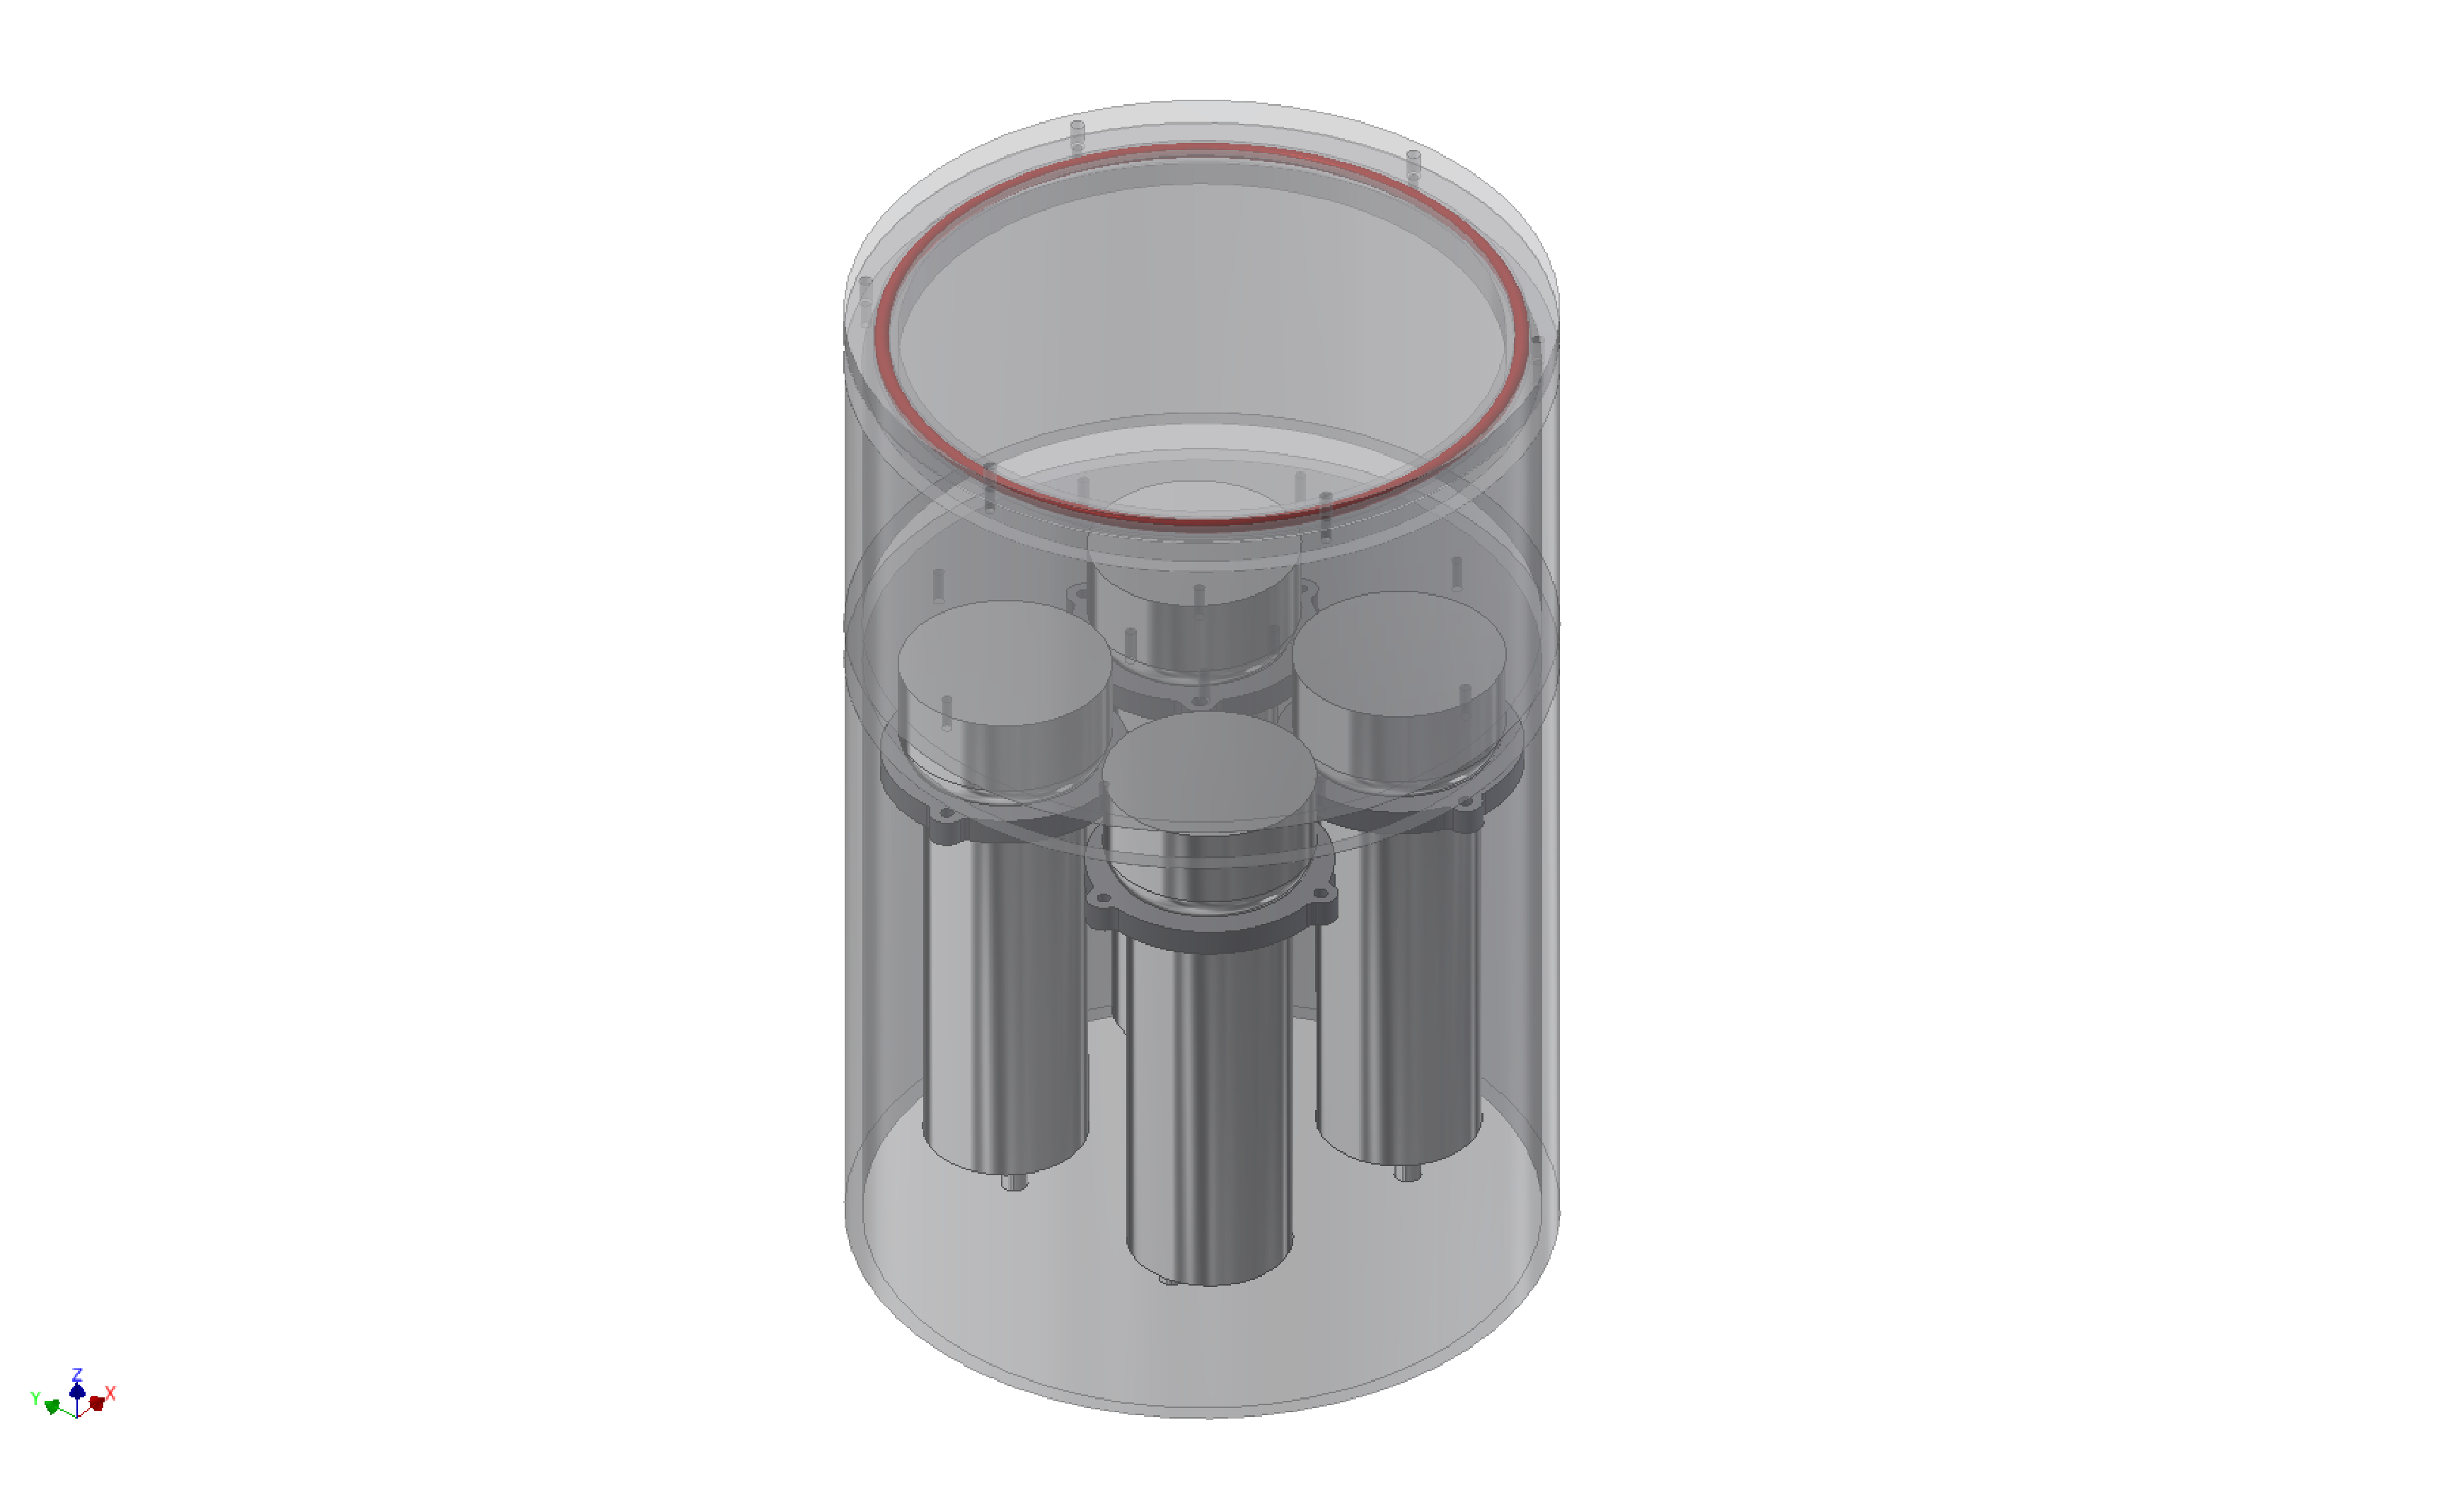
\includegraphics[width=\textwidth]{scout_vessel.pdf}
  \caption{3D Model of the acrylic vessel with 3 inch photomultipliers. The red ring is a silicone
  O-ring around the removable lid.}
\end{figure}
\begin{figure}
  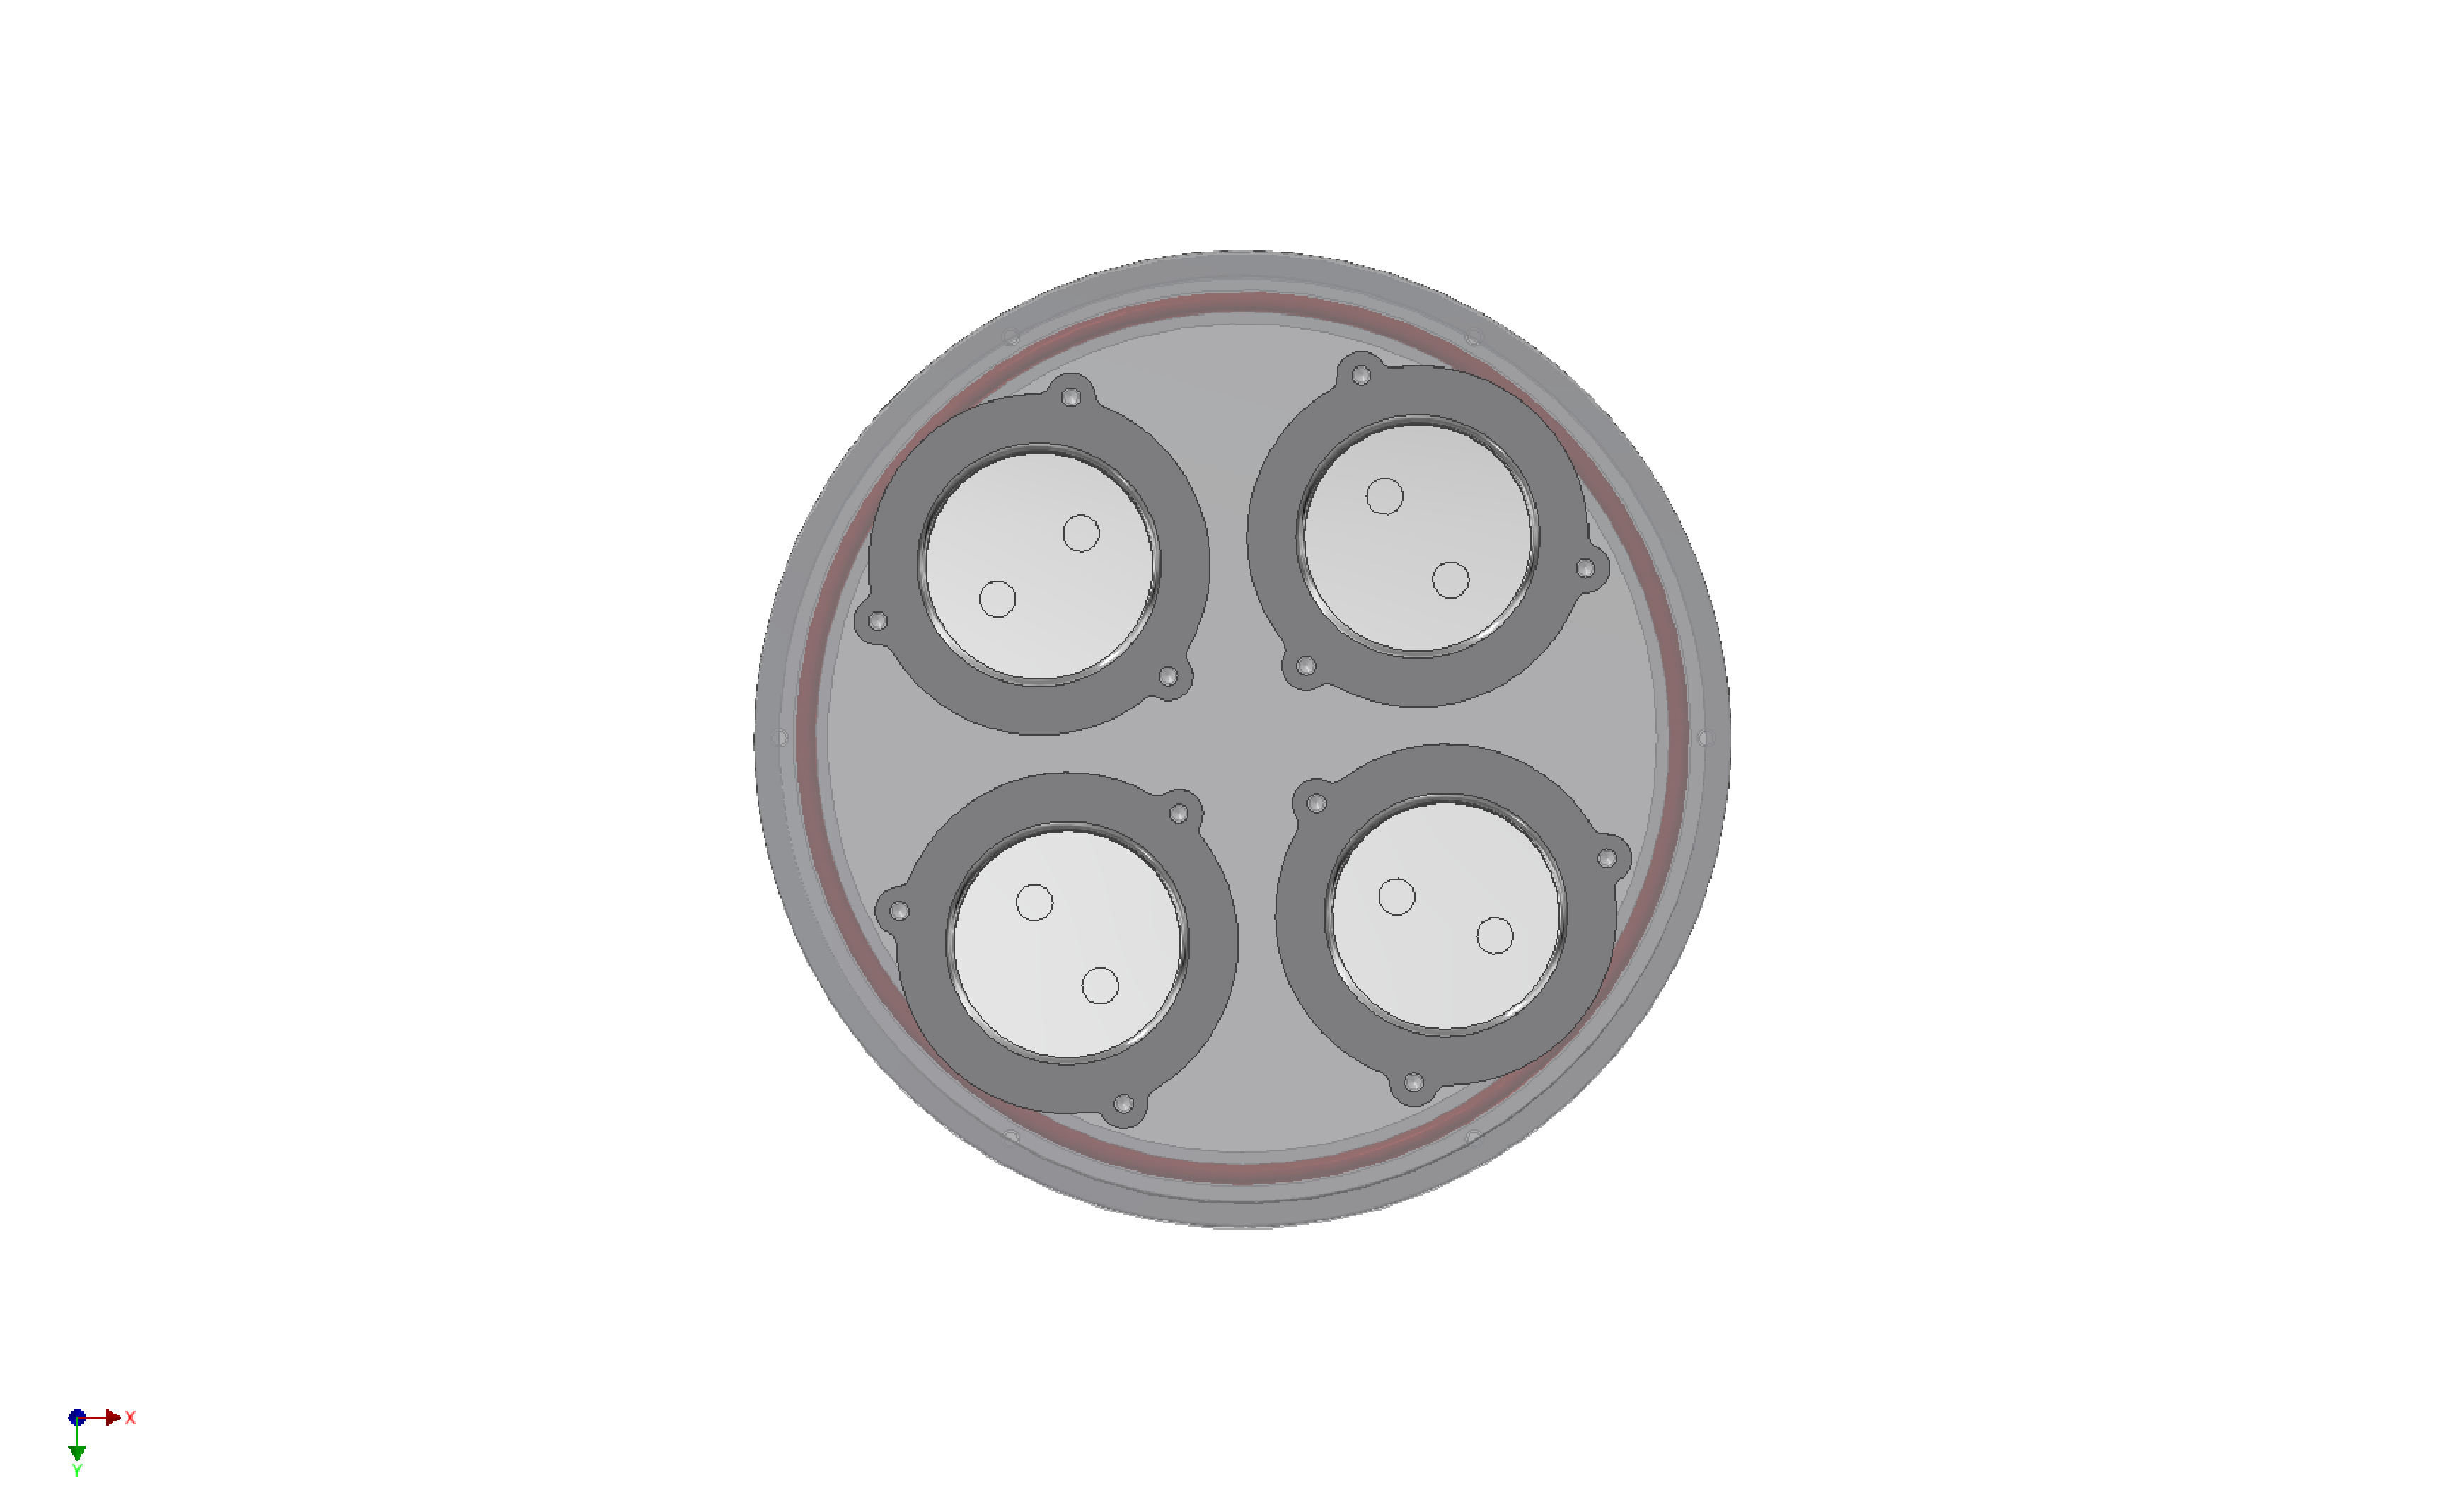
\includegraphics[width=\textwidth]{scout_vessel1.pdf}
  \caption{Top down view showing the photomultiplier foot-print looking into the acrylic vessel}
\end{figure}
\begin{figure}
  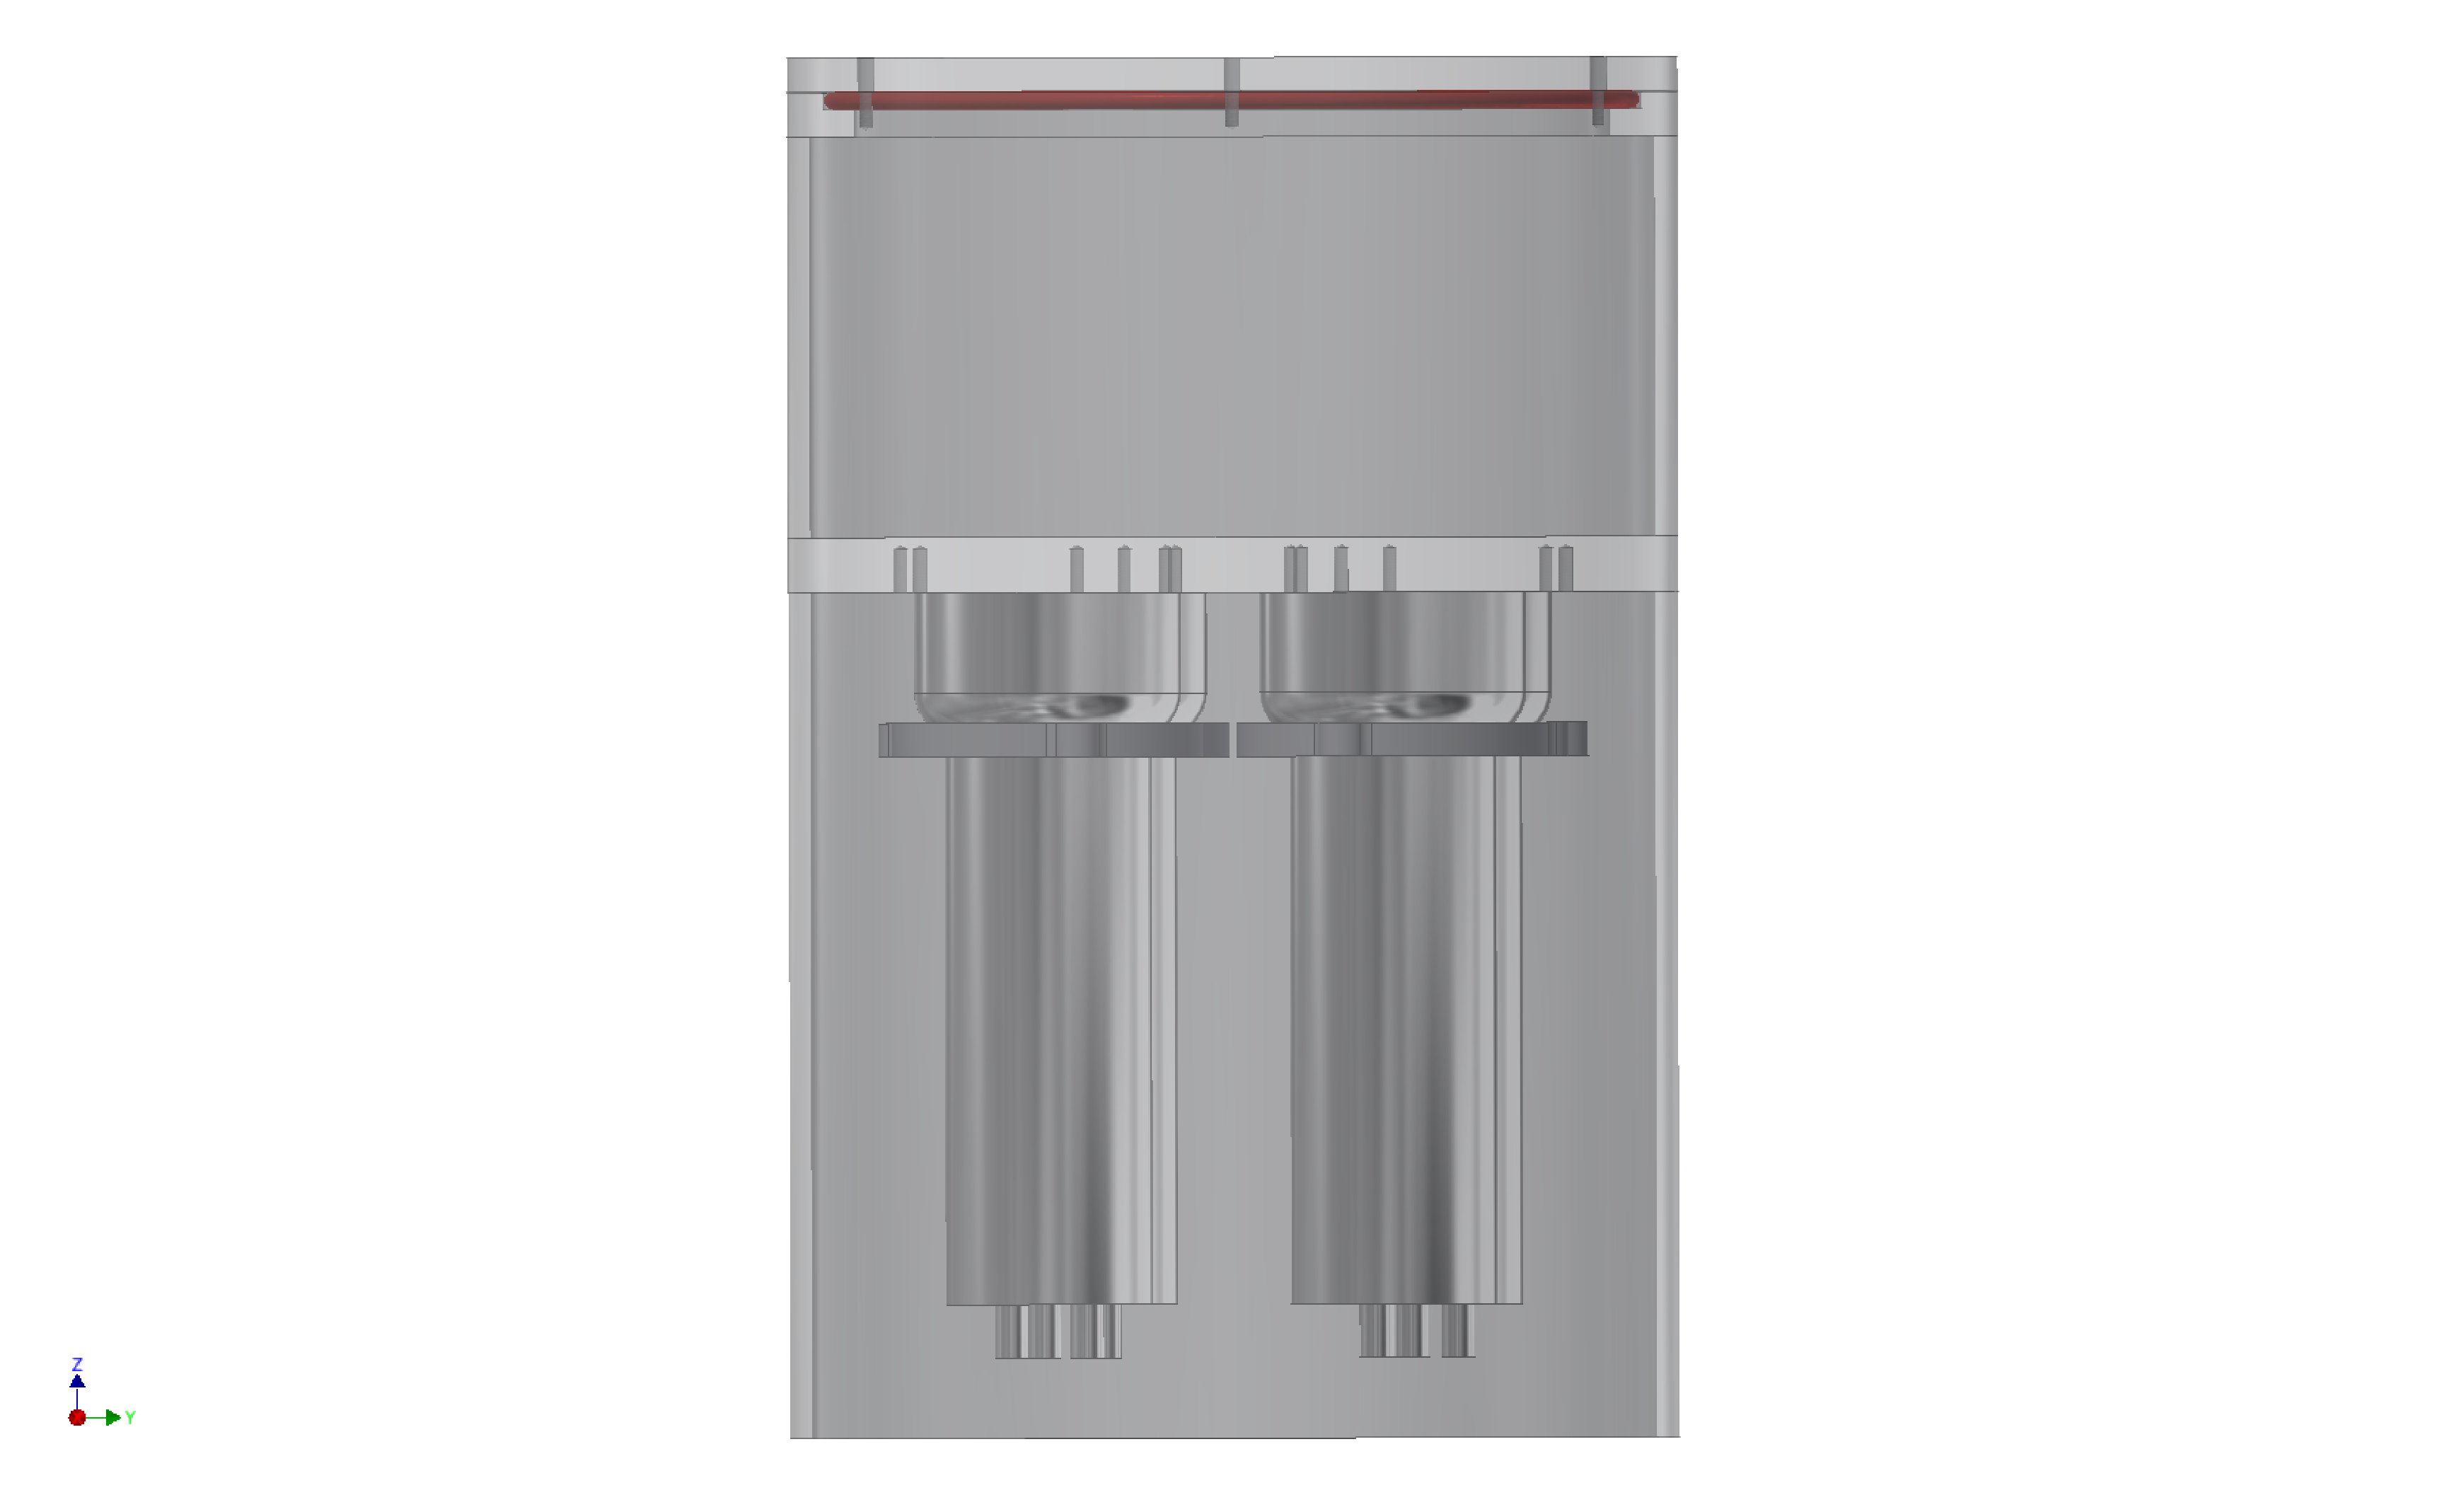
\includegraphics[width=\textwidth]{scout_vessel2.pdf}
  \caption{Scout as seen from the side.}
\end{figure}
\begin{figure}
  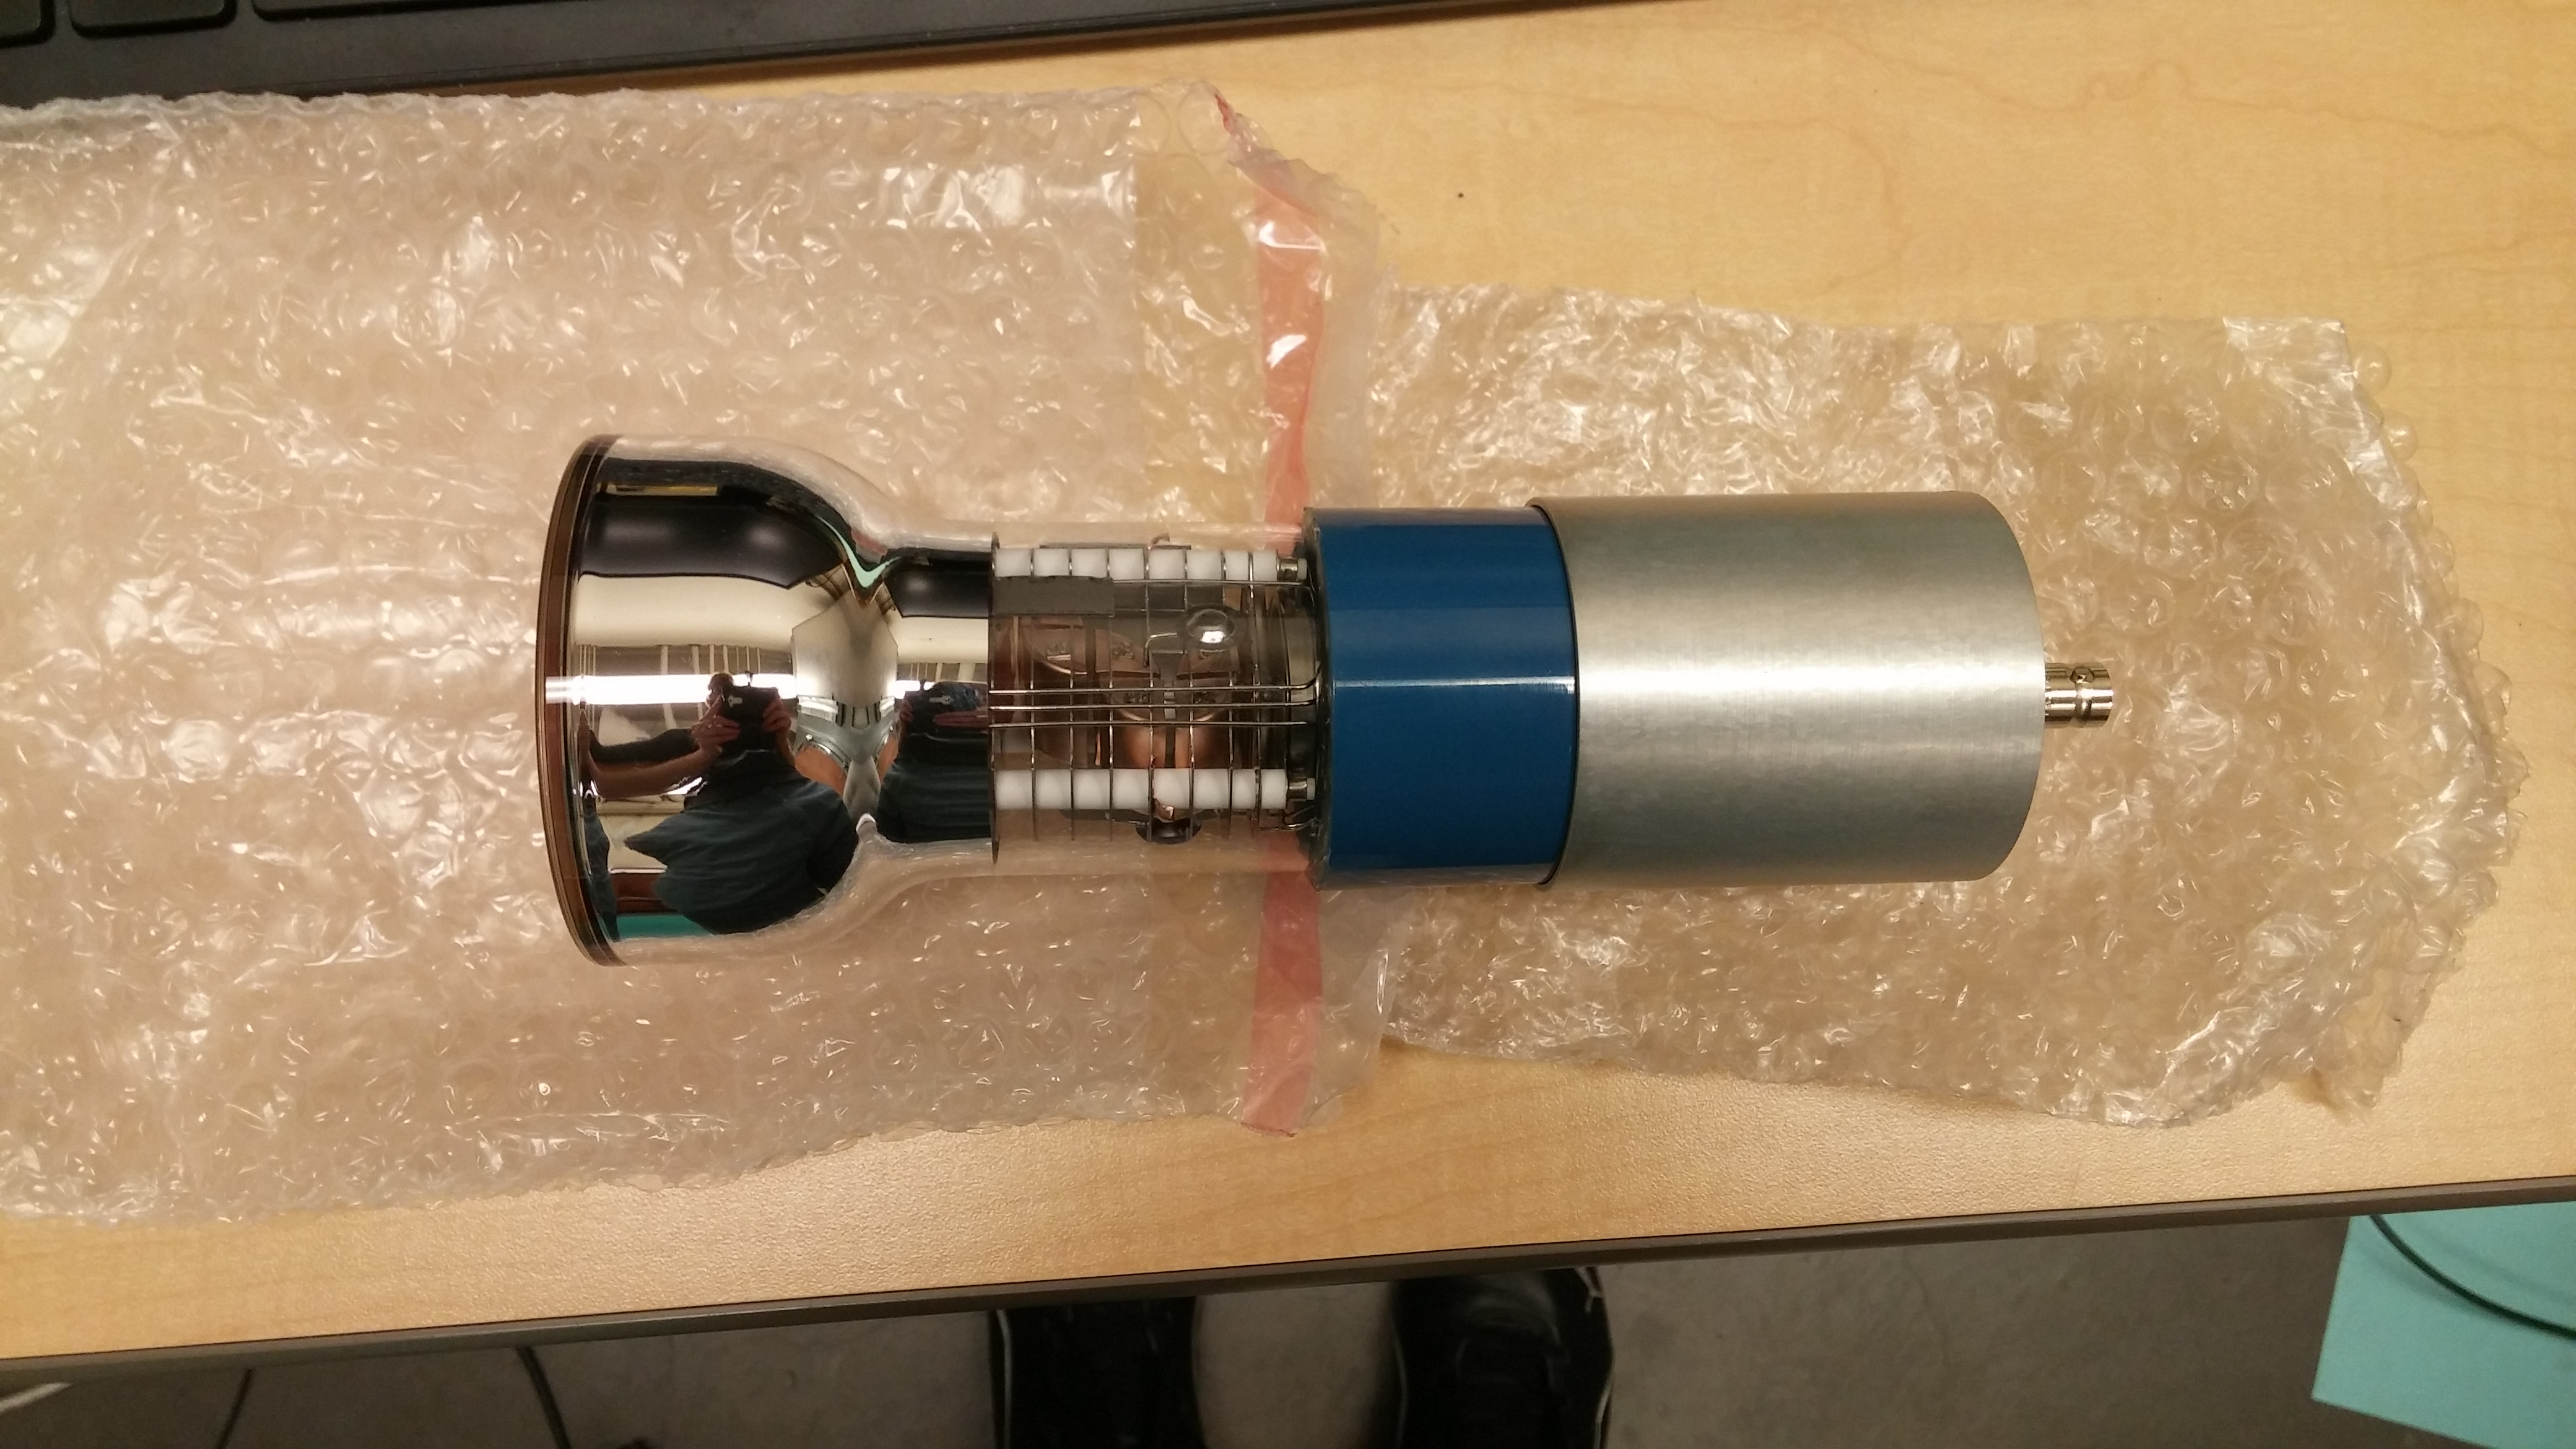
\includegraphics[width=\textwidth]{adit_pmt.jpg}
  \caption{3 inch ADIT photomultiplier}
\end{figure}
\begin{figure}
  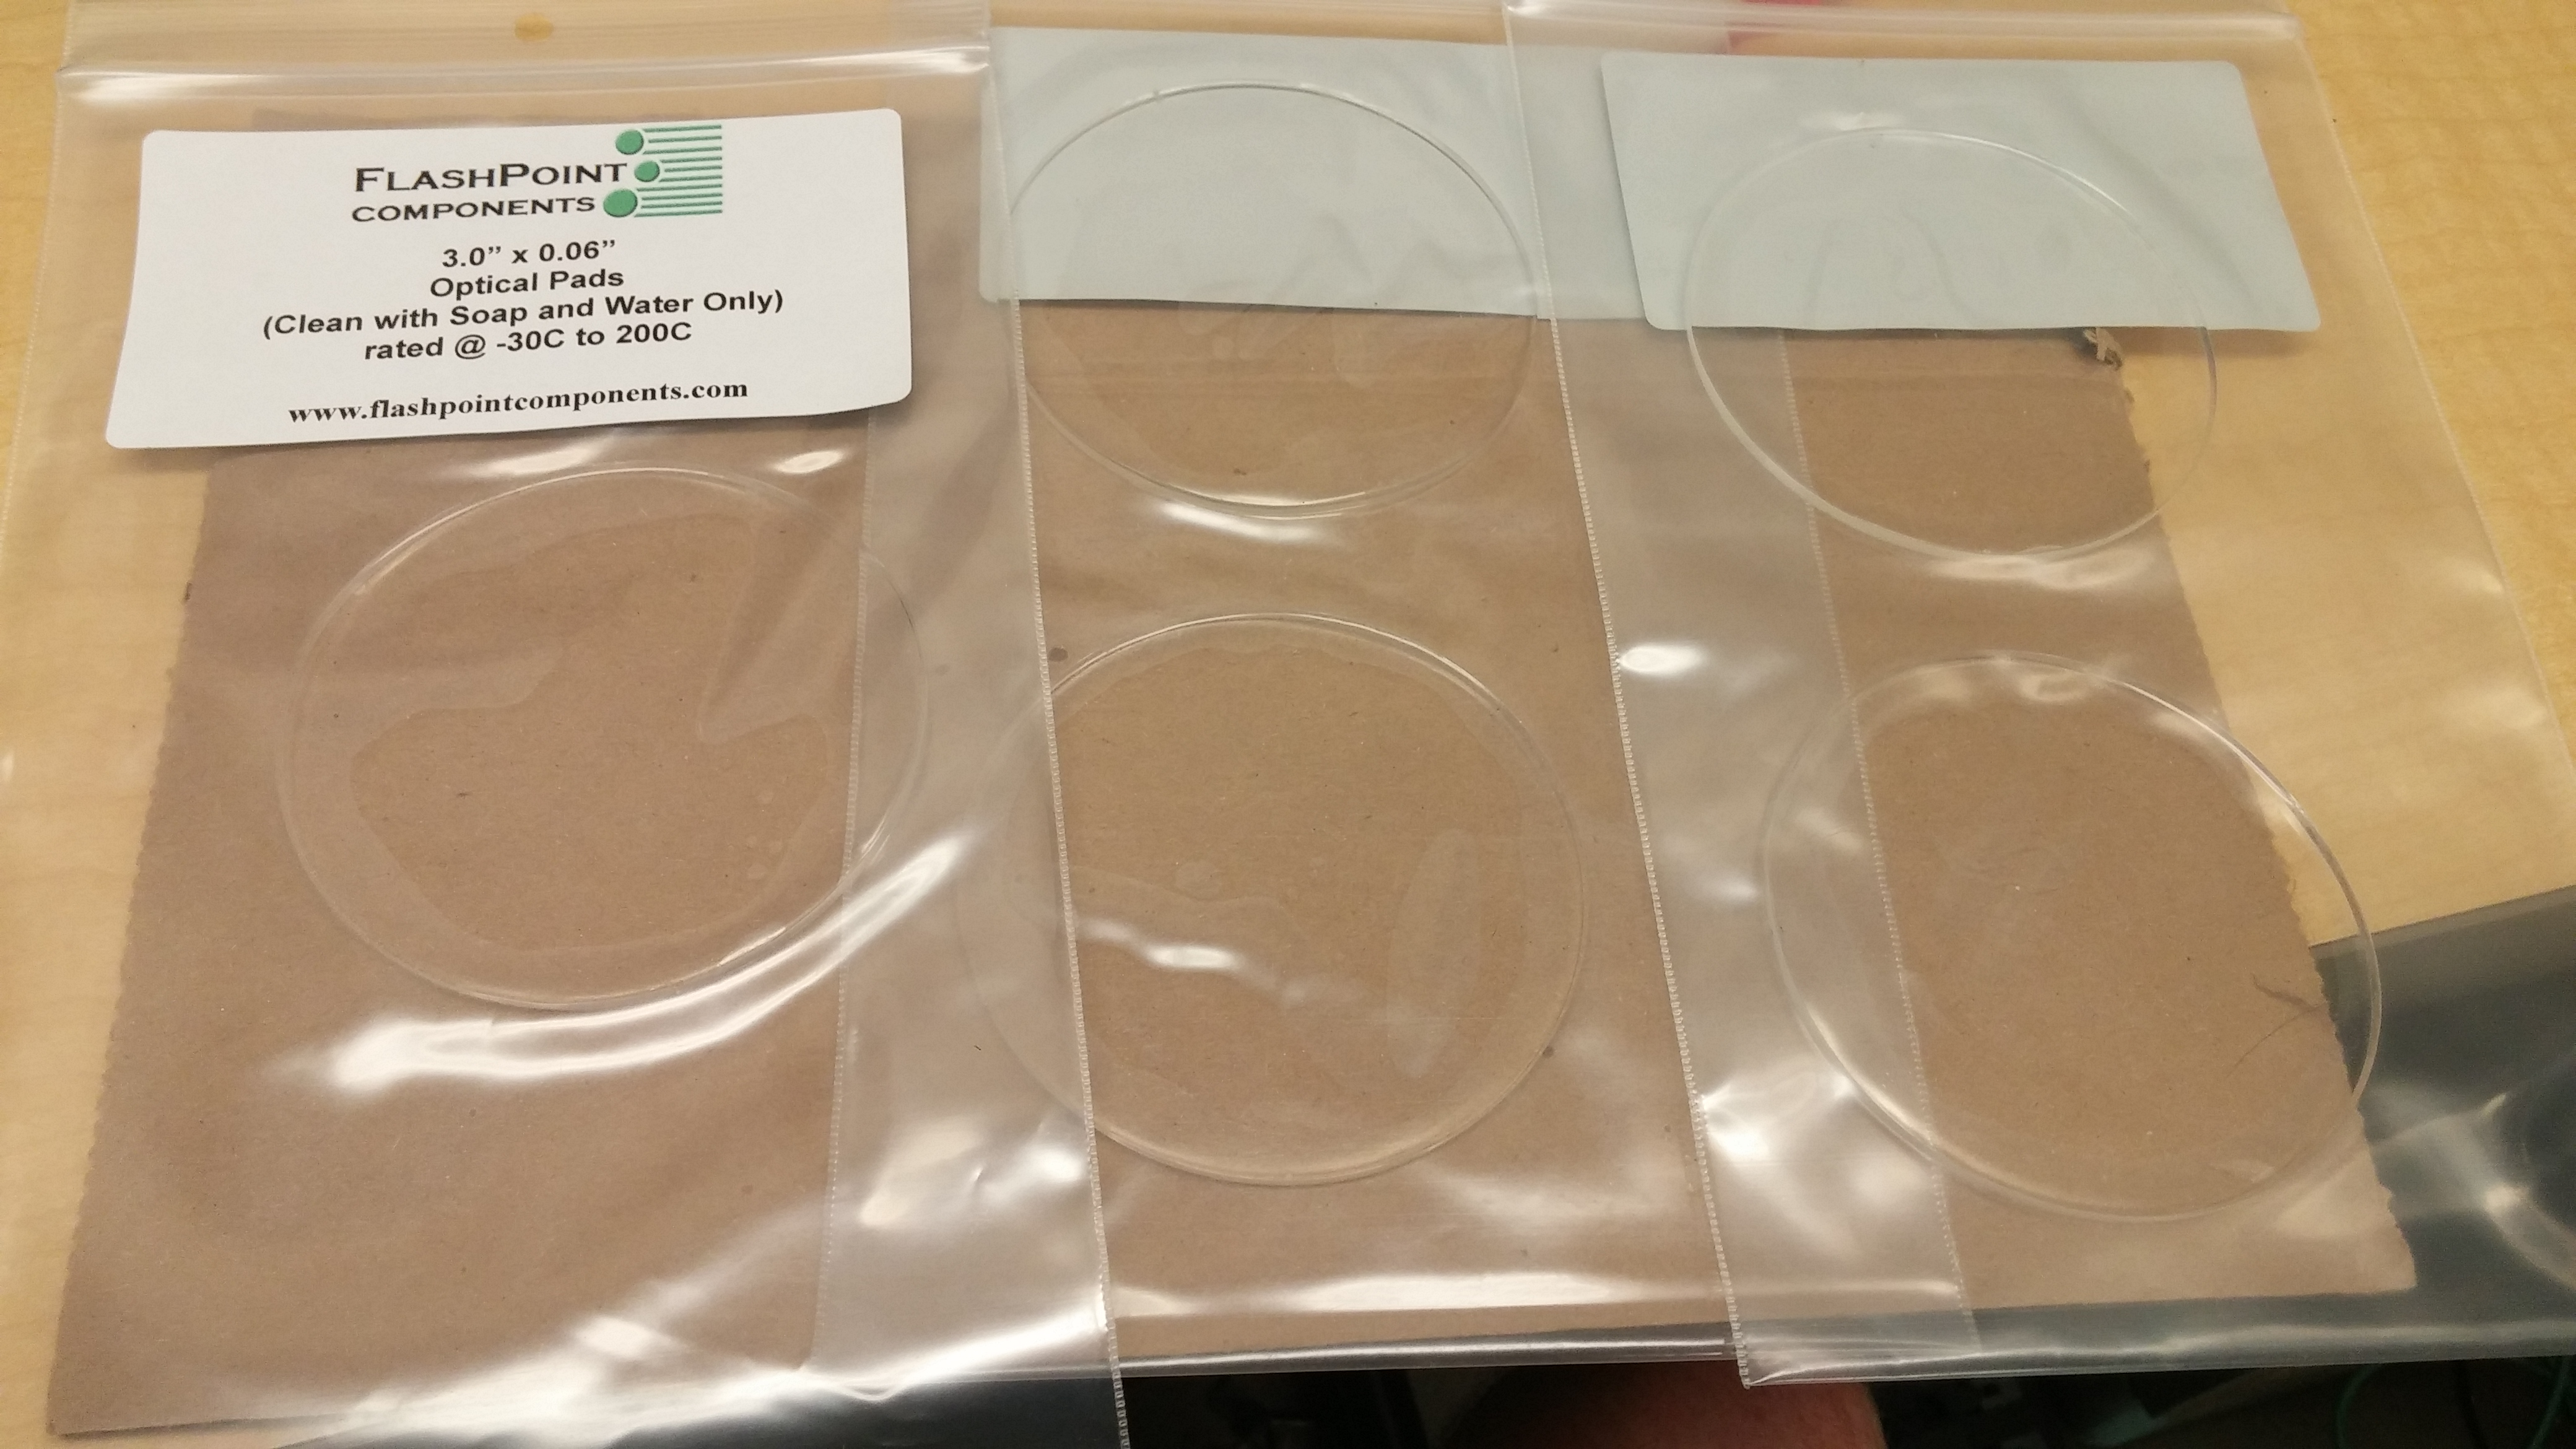
\includegraphics[width=\textwidth]{optical_pads.jpg}
  \caption{Flashpoint optical coupling pads, used in place of optical grease,
  to couple the photomultipliers with the bottom of the acrylic vessel}
\end{figure}
\begin{figure}
  \centering
  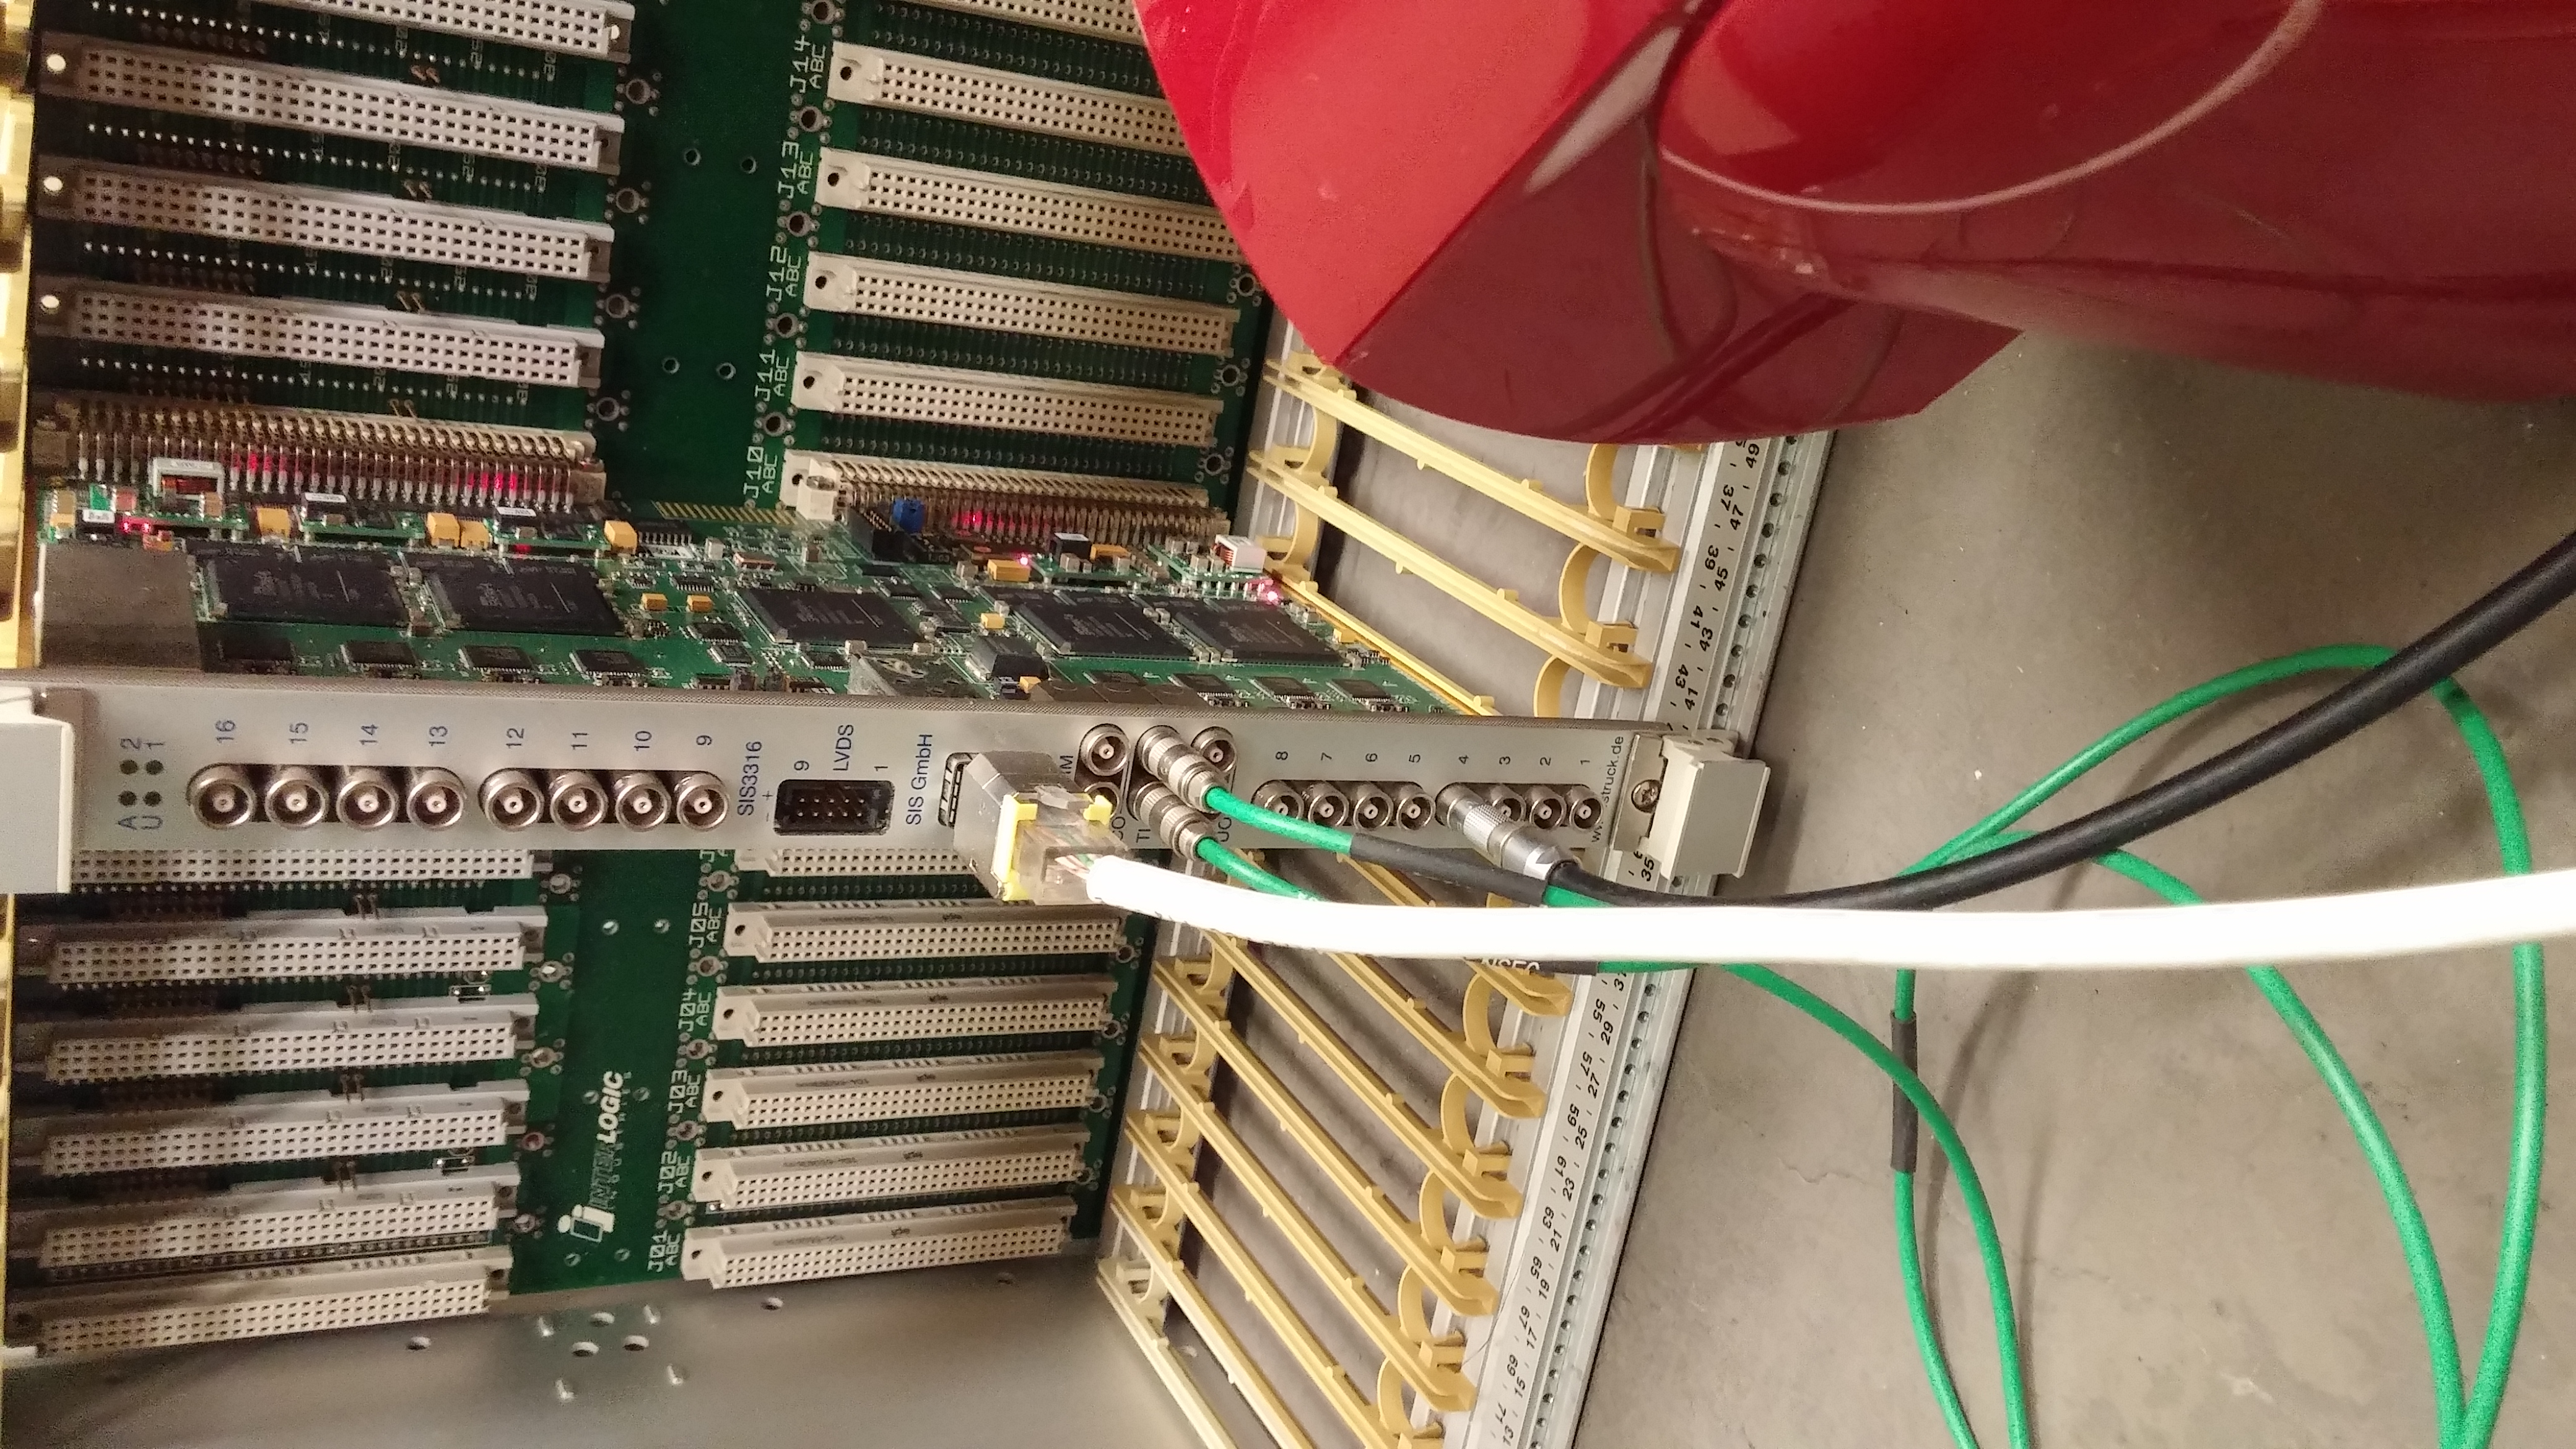
\includegraphics[width=\textwidth, angle=270]{sis3316.jpg}
  \caption{Struck SIS3316 16 channel 250 MS/s 14-bit digitizer with an ethernet SFP cage
  used for programming and data collection}
\end{figure}
\begin{figure}
  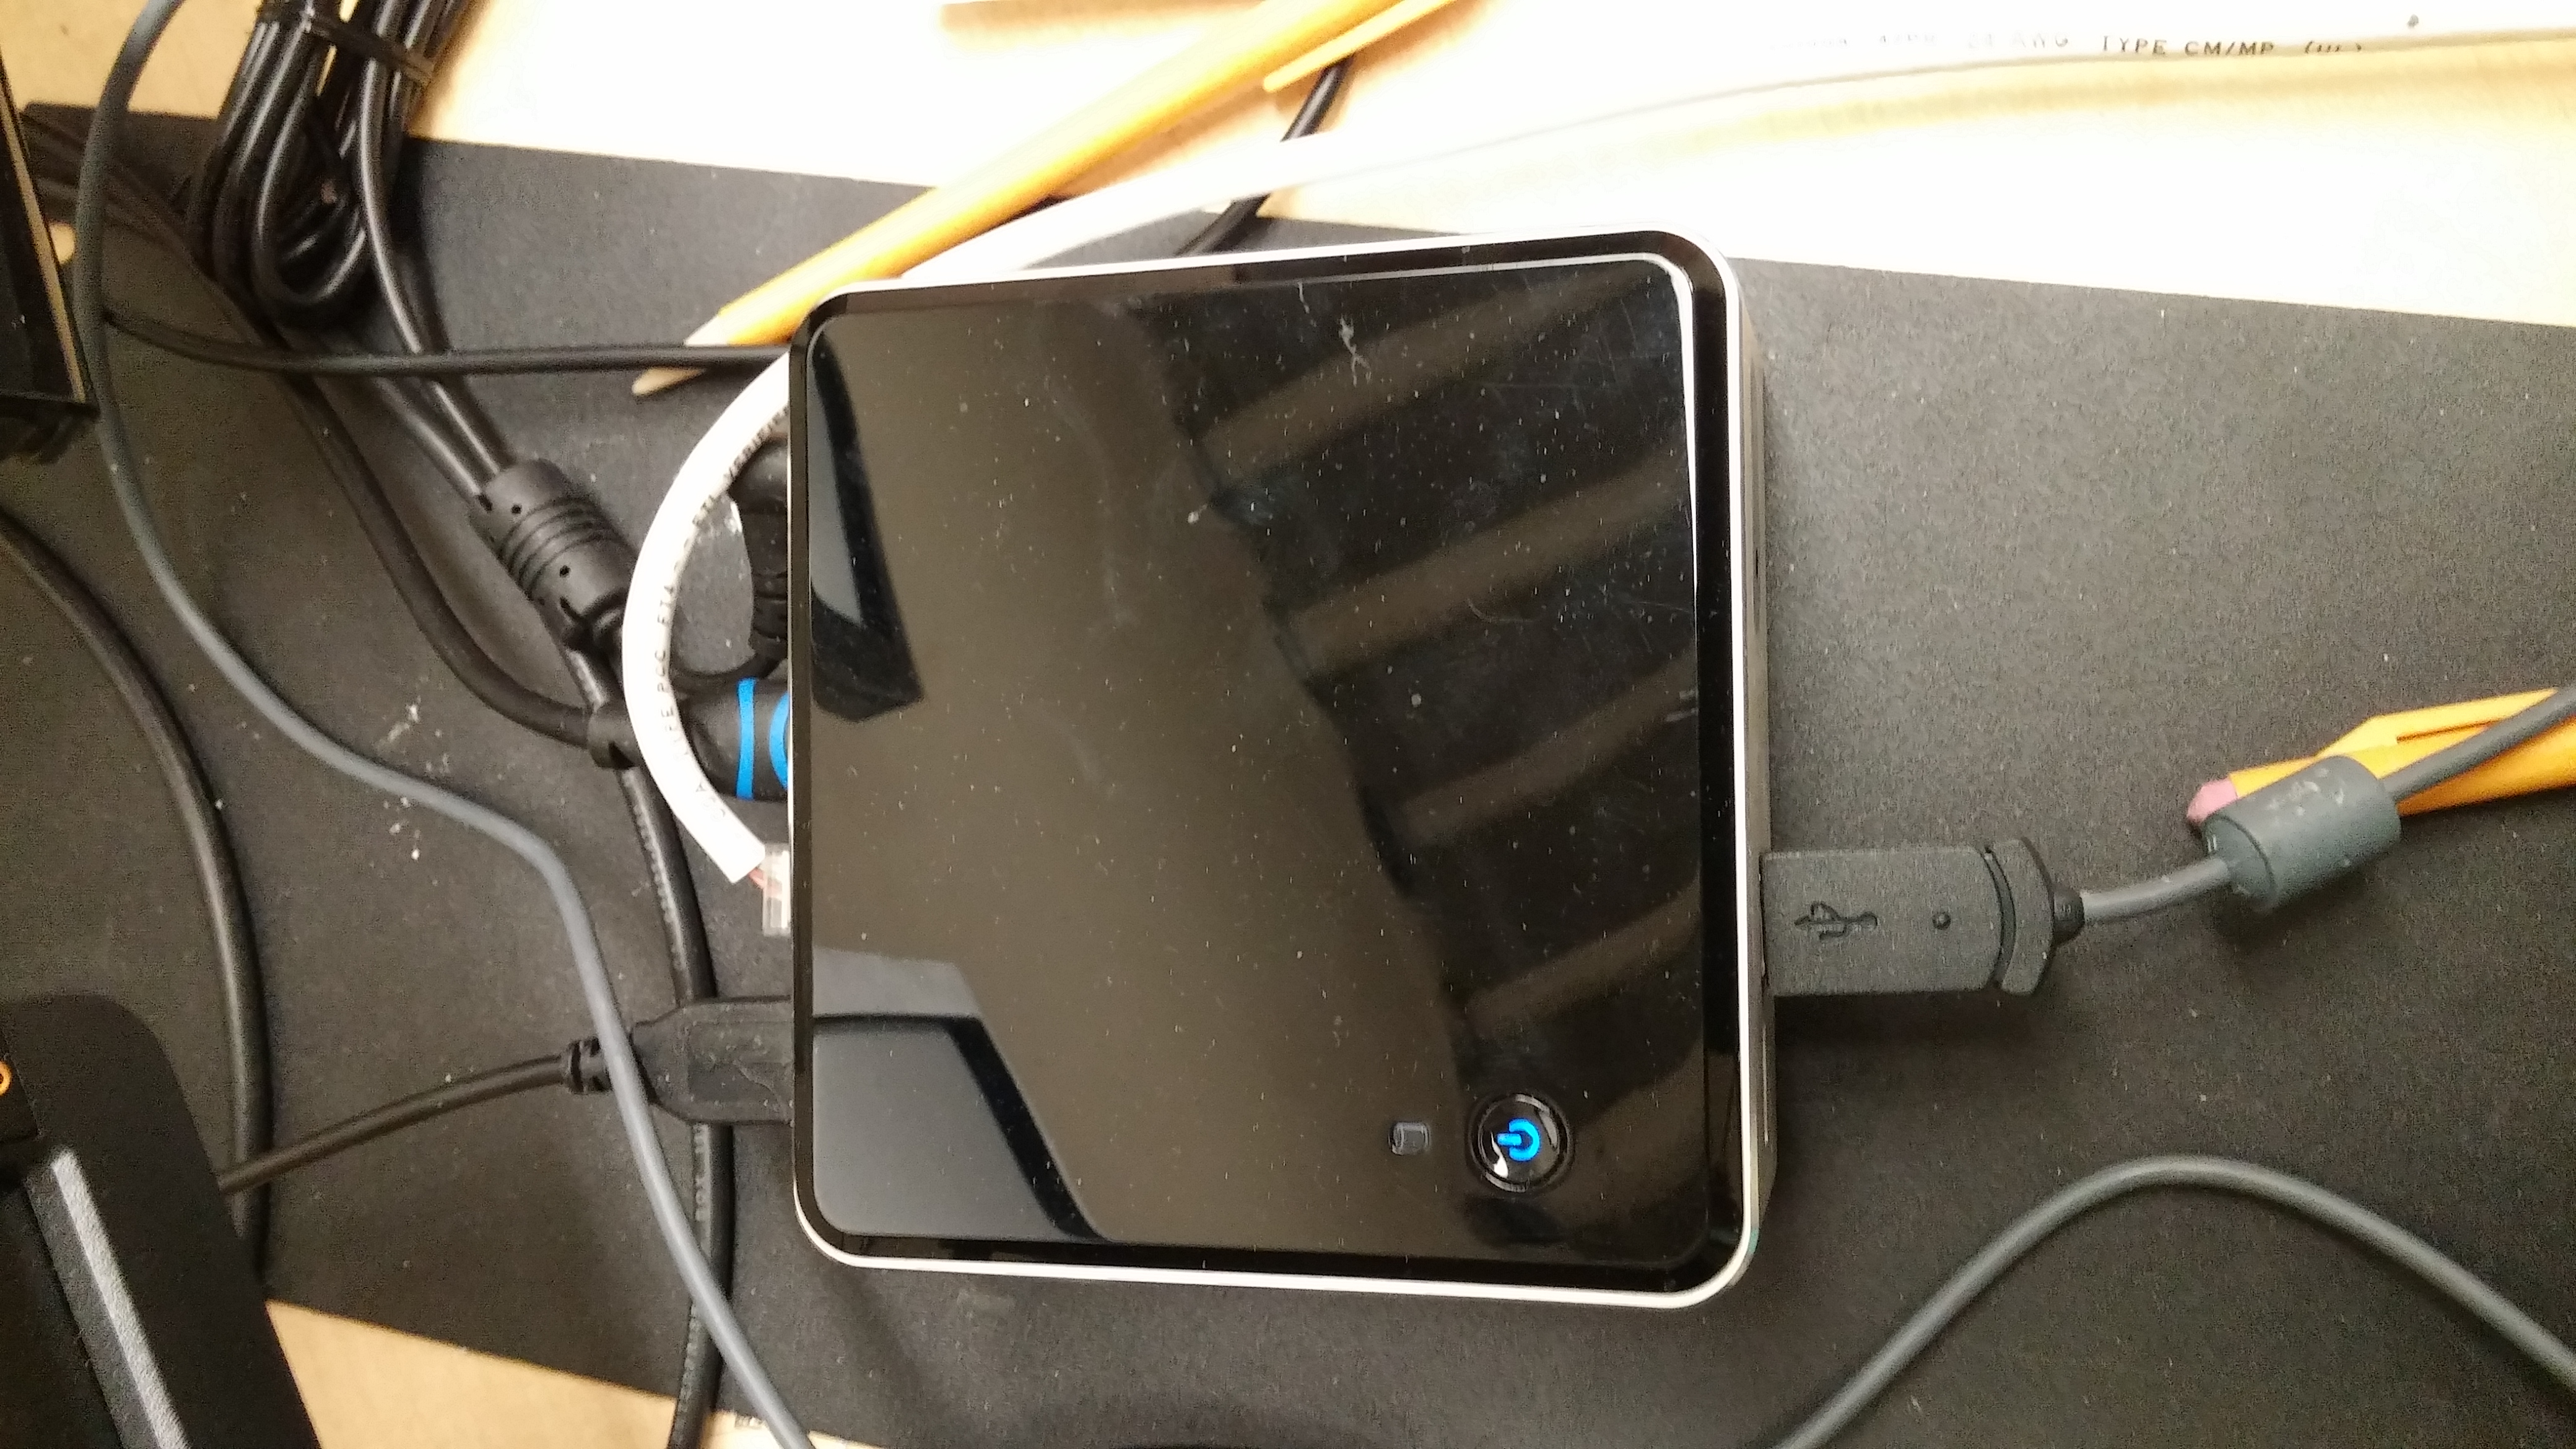
\includegraphics[width=\textwidth]{nuc.jpg}
  \caption{Intel NUC which records the data from the digitizer via an ethernet connection}
\end{figure}
\begin{figure}
  \centering
  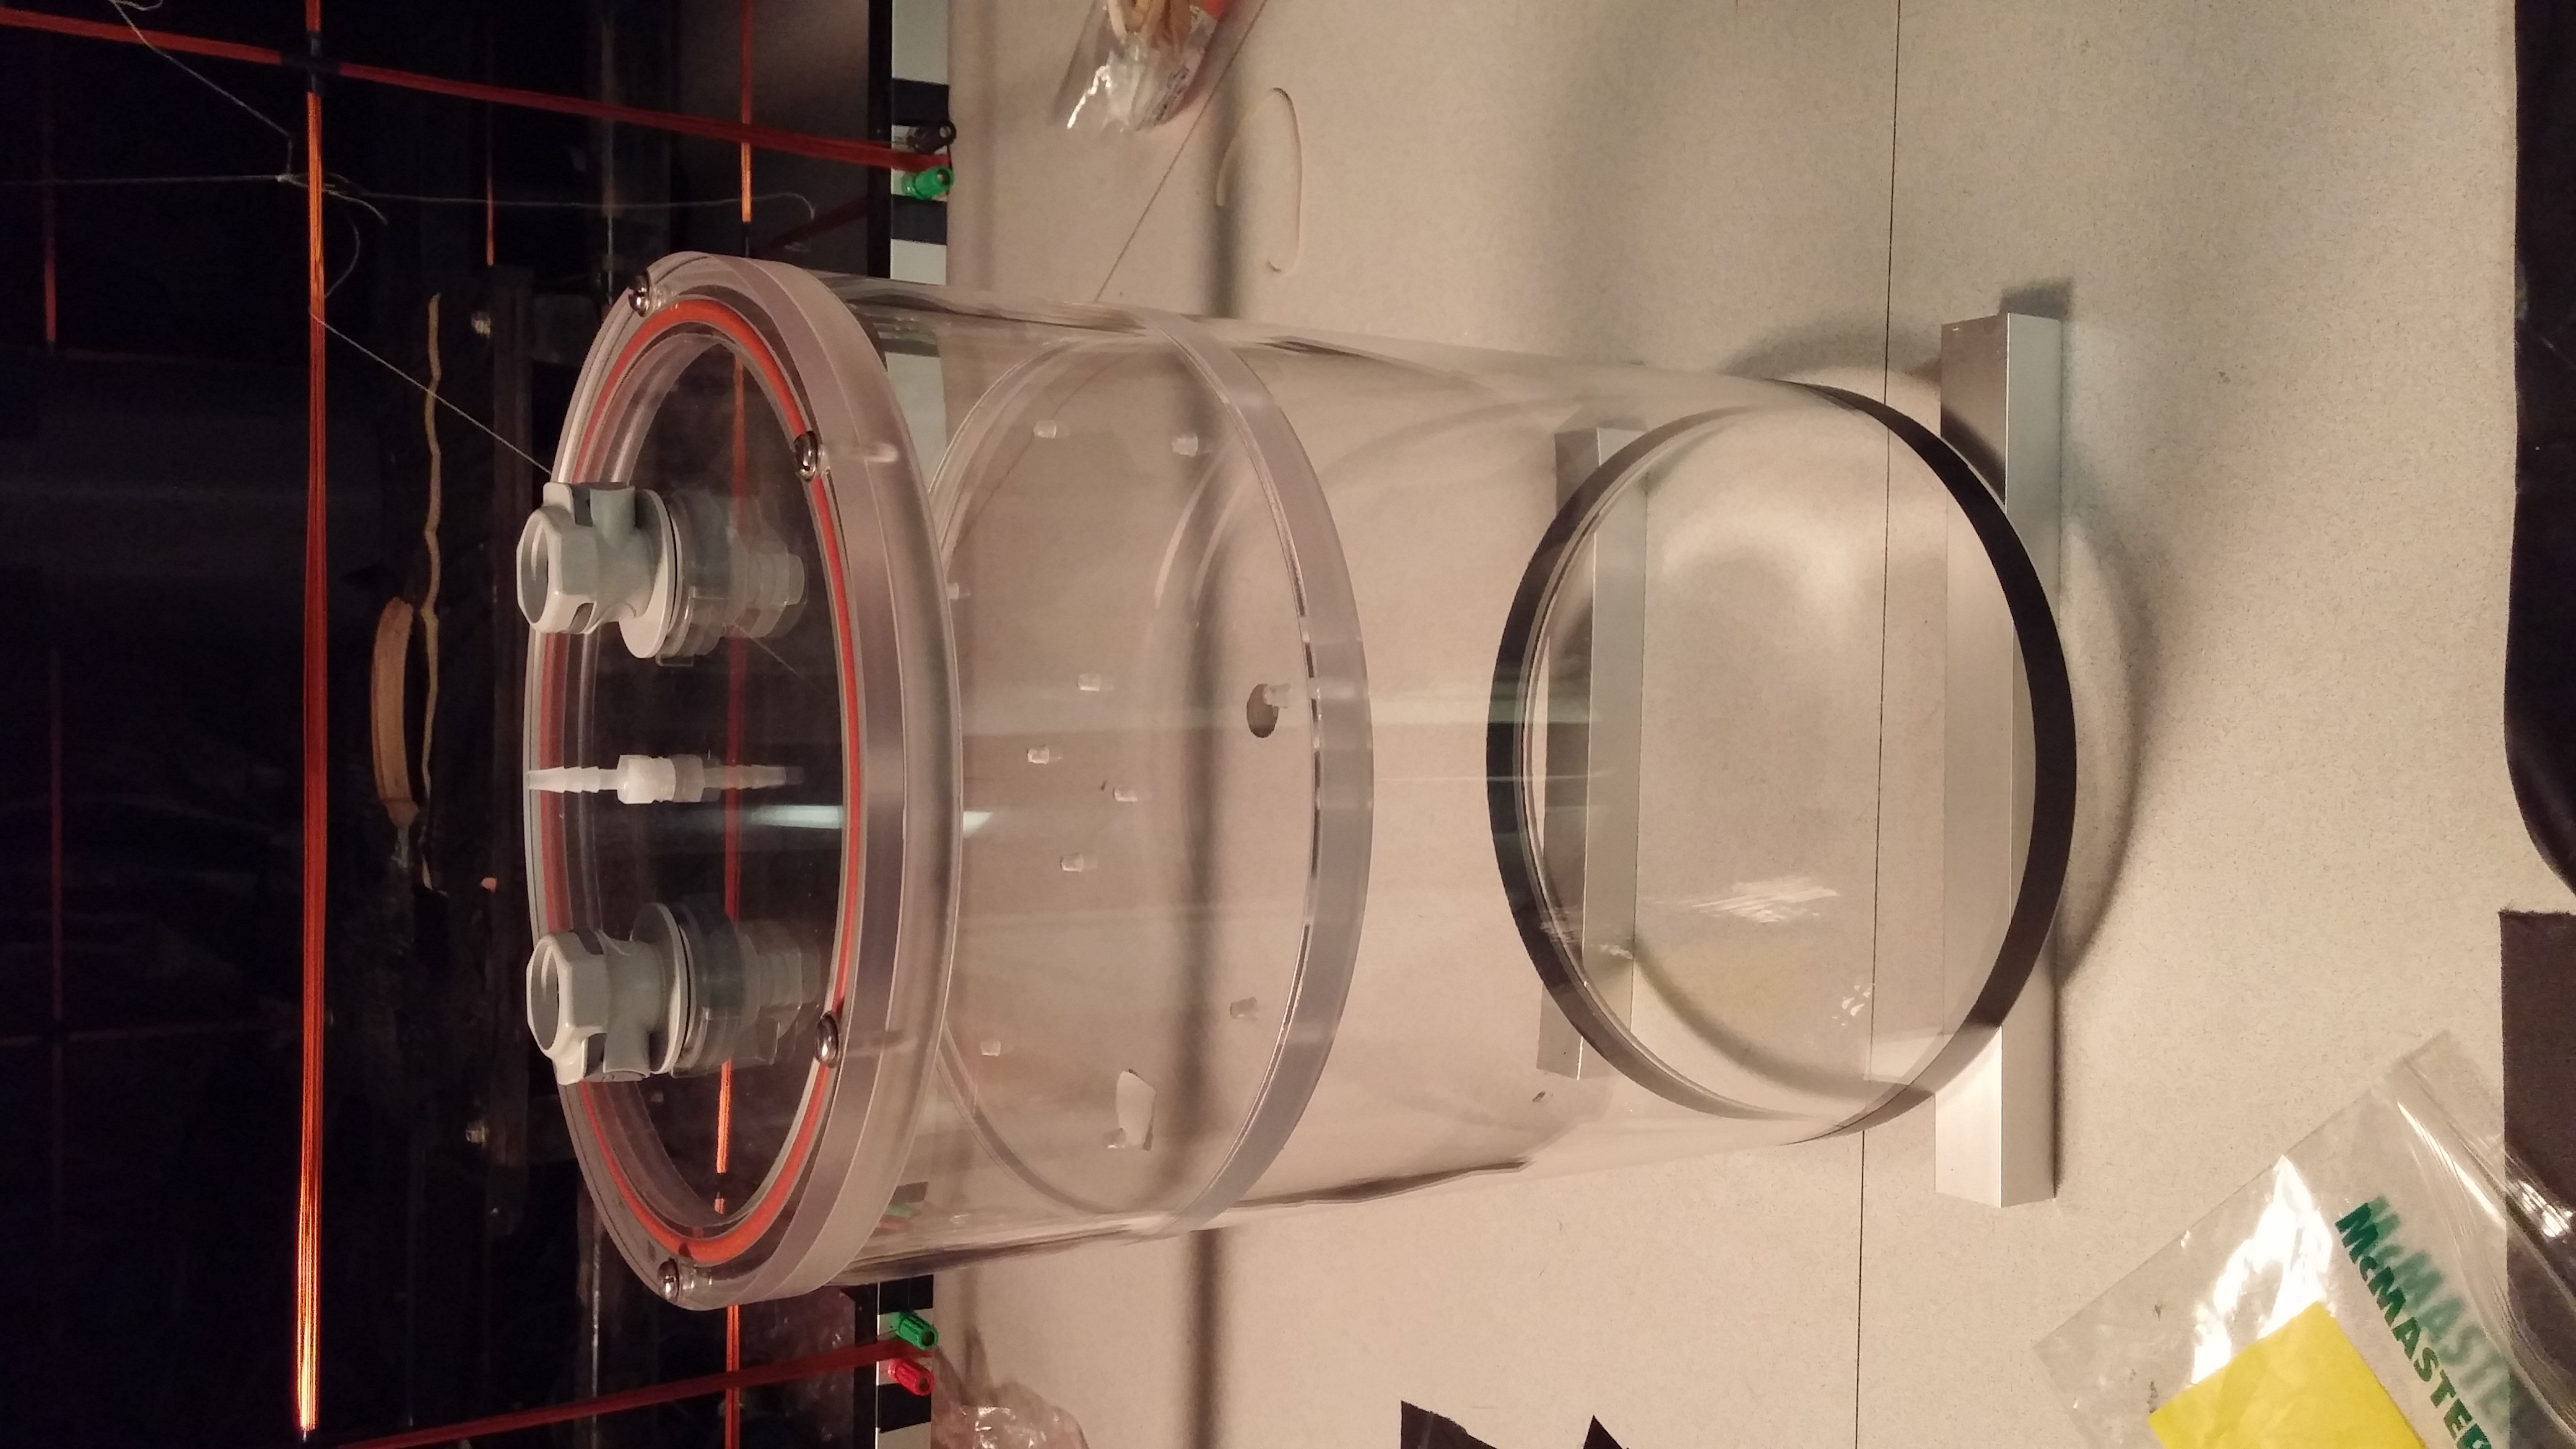
\includegraphics[width=\textwidth, angle=270]{real_scout.jpg}
  \caption{Scout acrylic vessel with a 0.5 psi check valve (small white port in the center
  of the lid), and two quick-disconnects for fluid/gas transfer. The lid is removed via the
  6 flat-head screws around the top for easy cleaning.}
\end{figure}
\begin{figure}
  \centering
  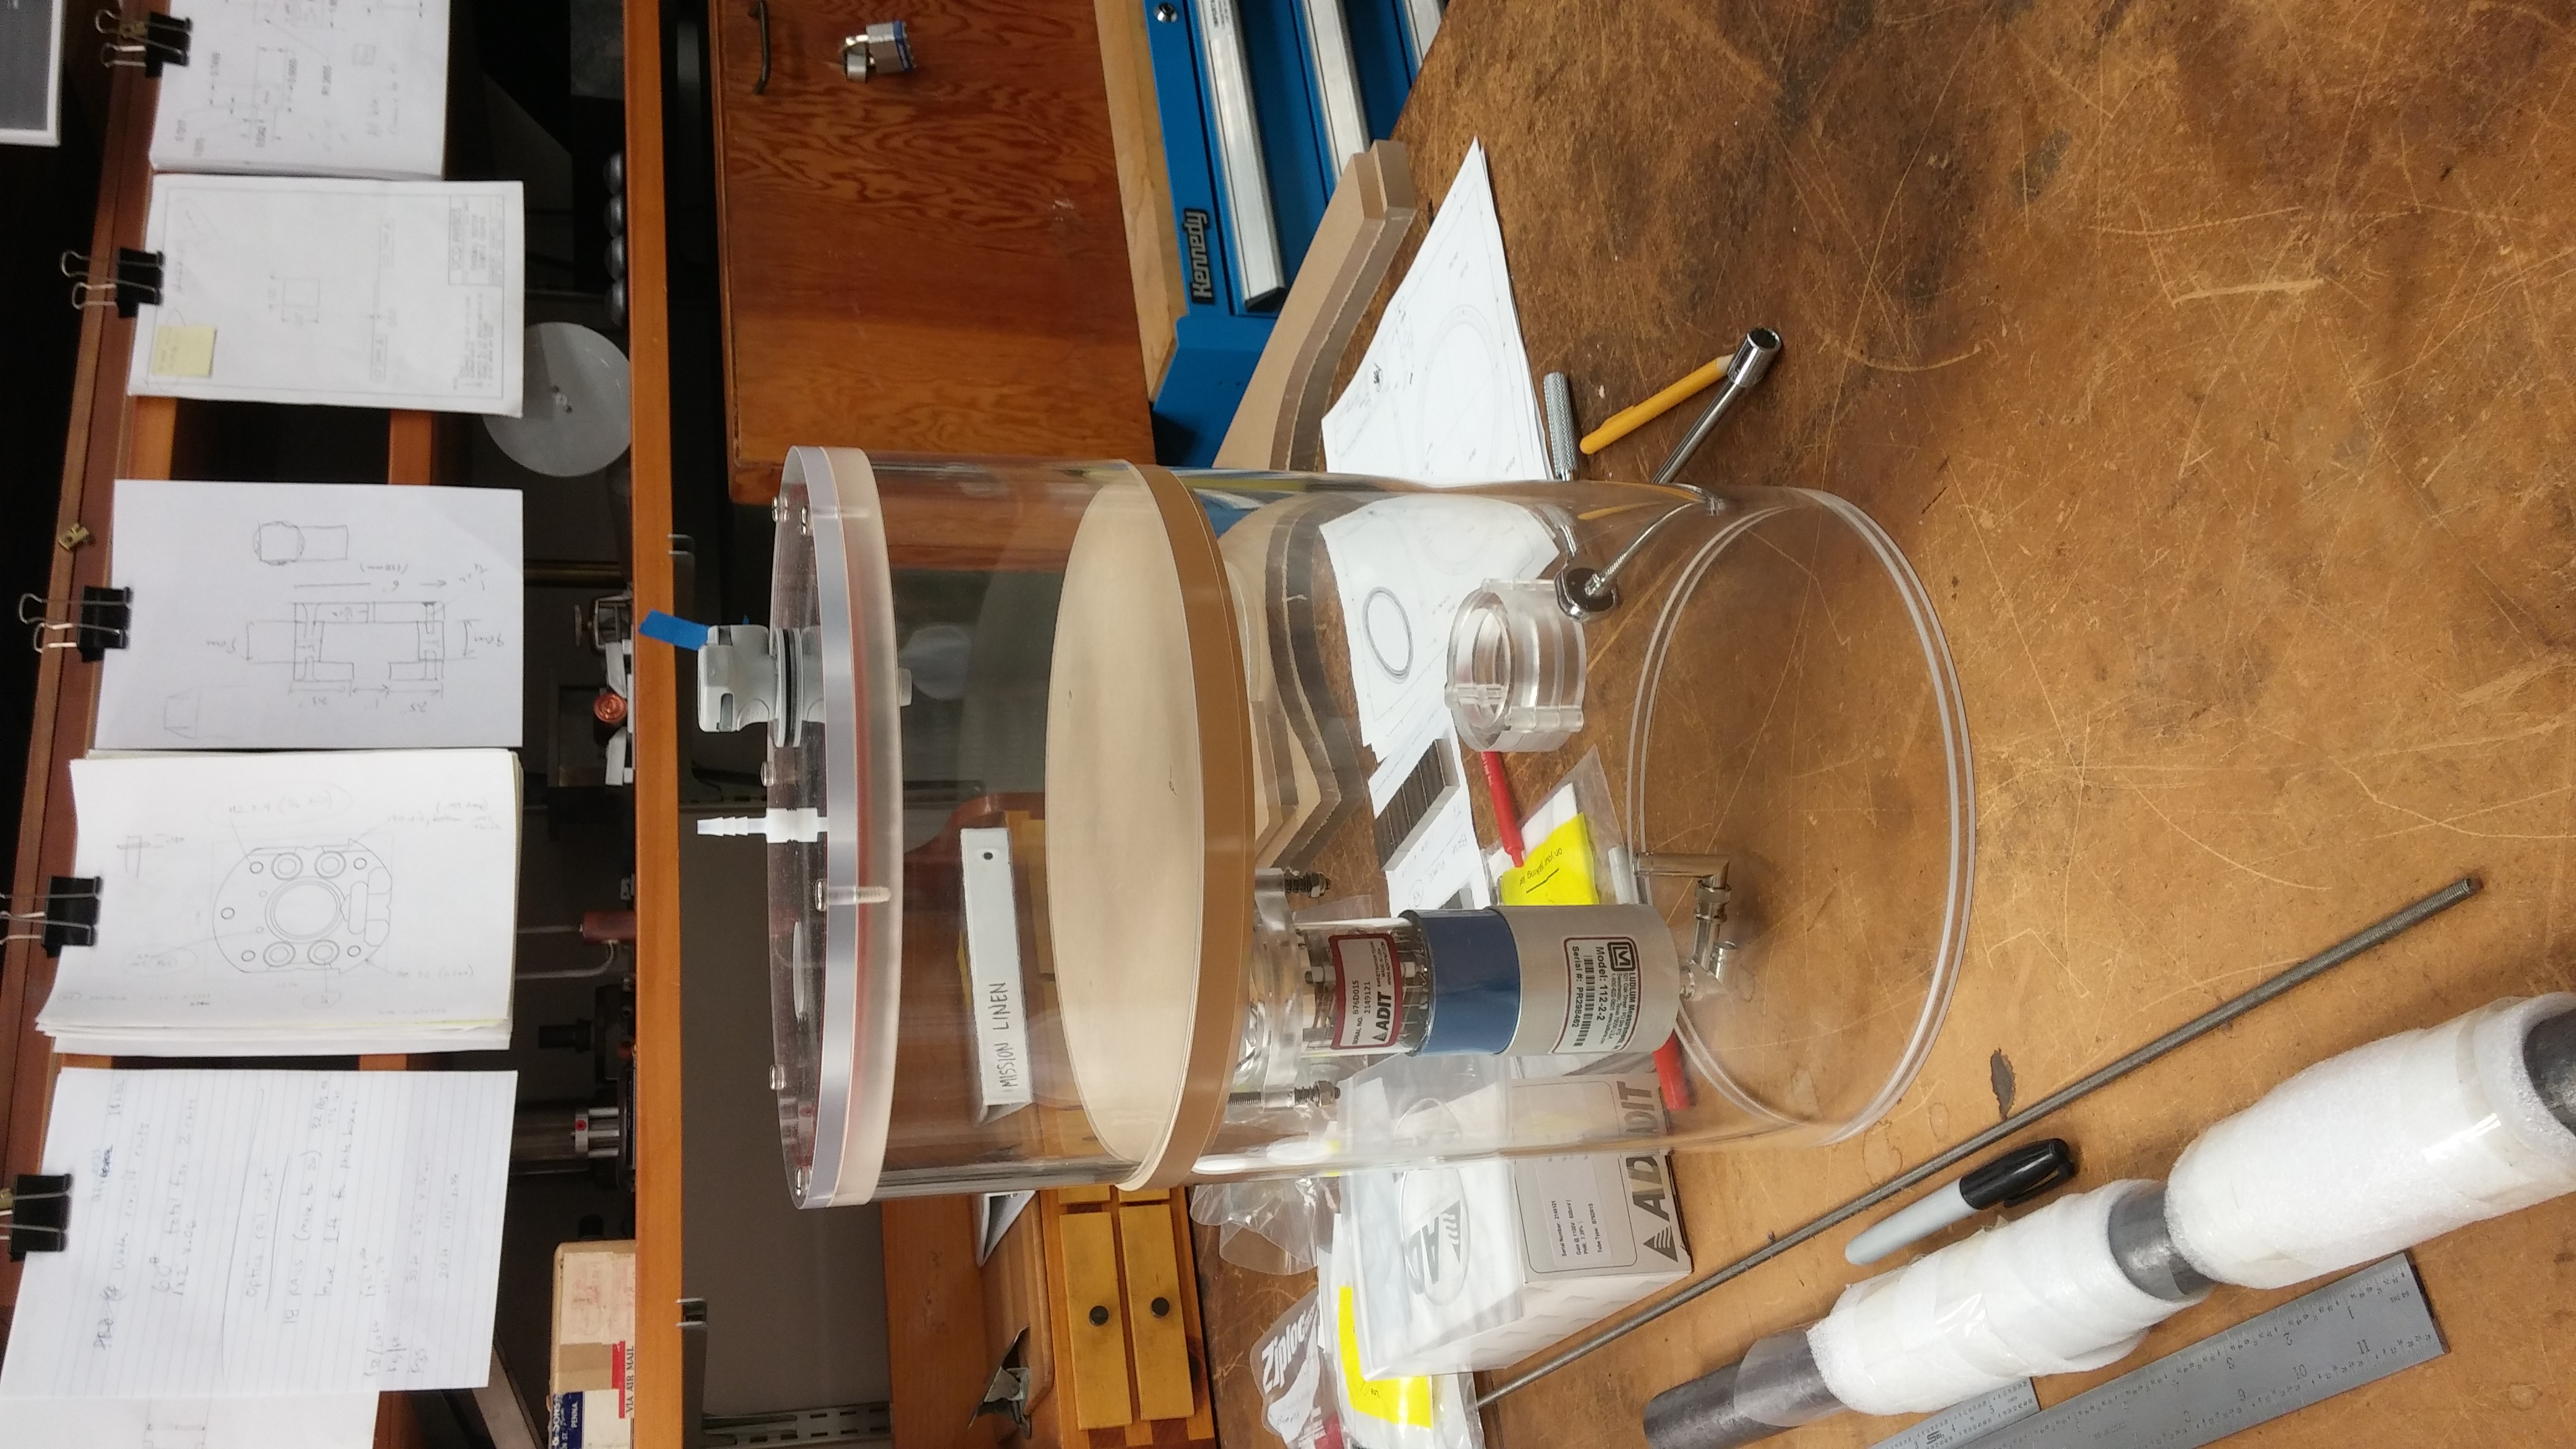
\includegraphics[width=\textwidth, angle=270]{scout_construction.jpg}
  \caption{Scout with a single photomultiplier attached at the bottom demonstrating how it
  is held in place and the total clearance at the bottom.}
\end{figure}
\begin{figure}
  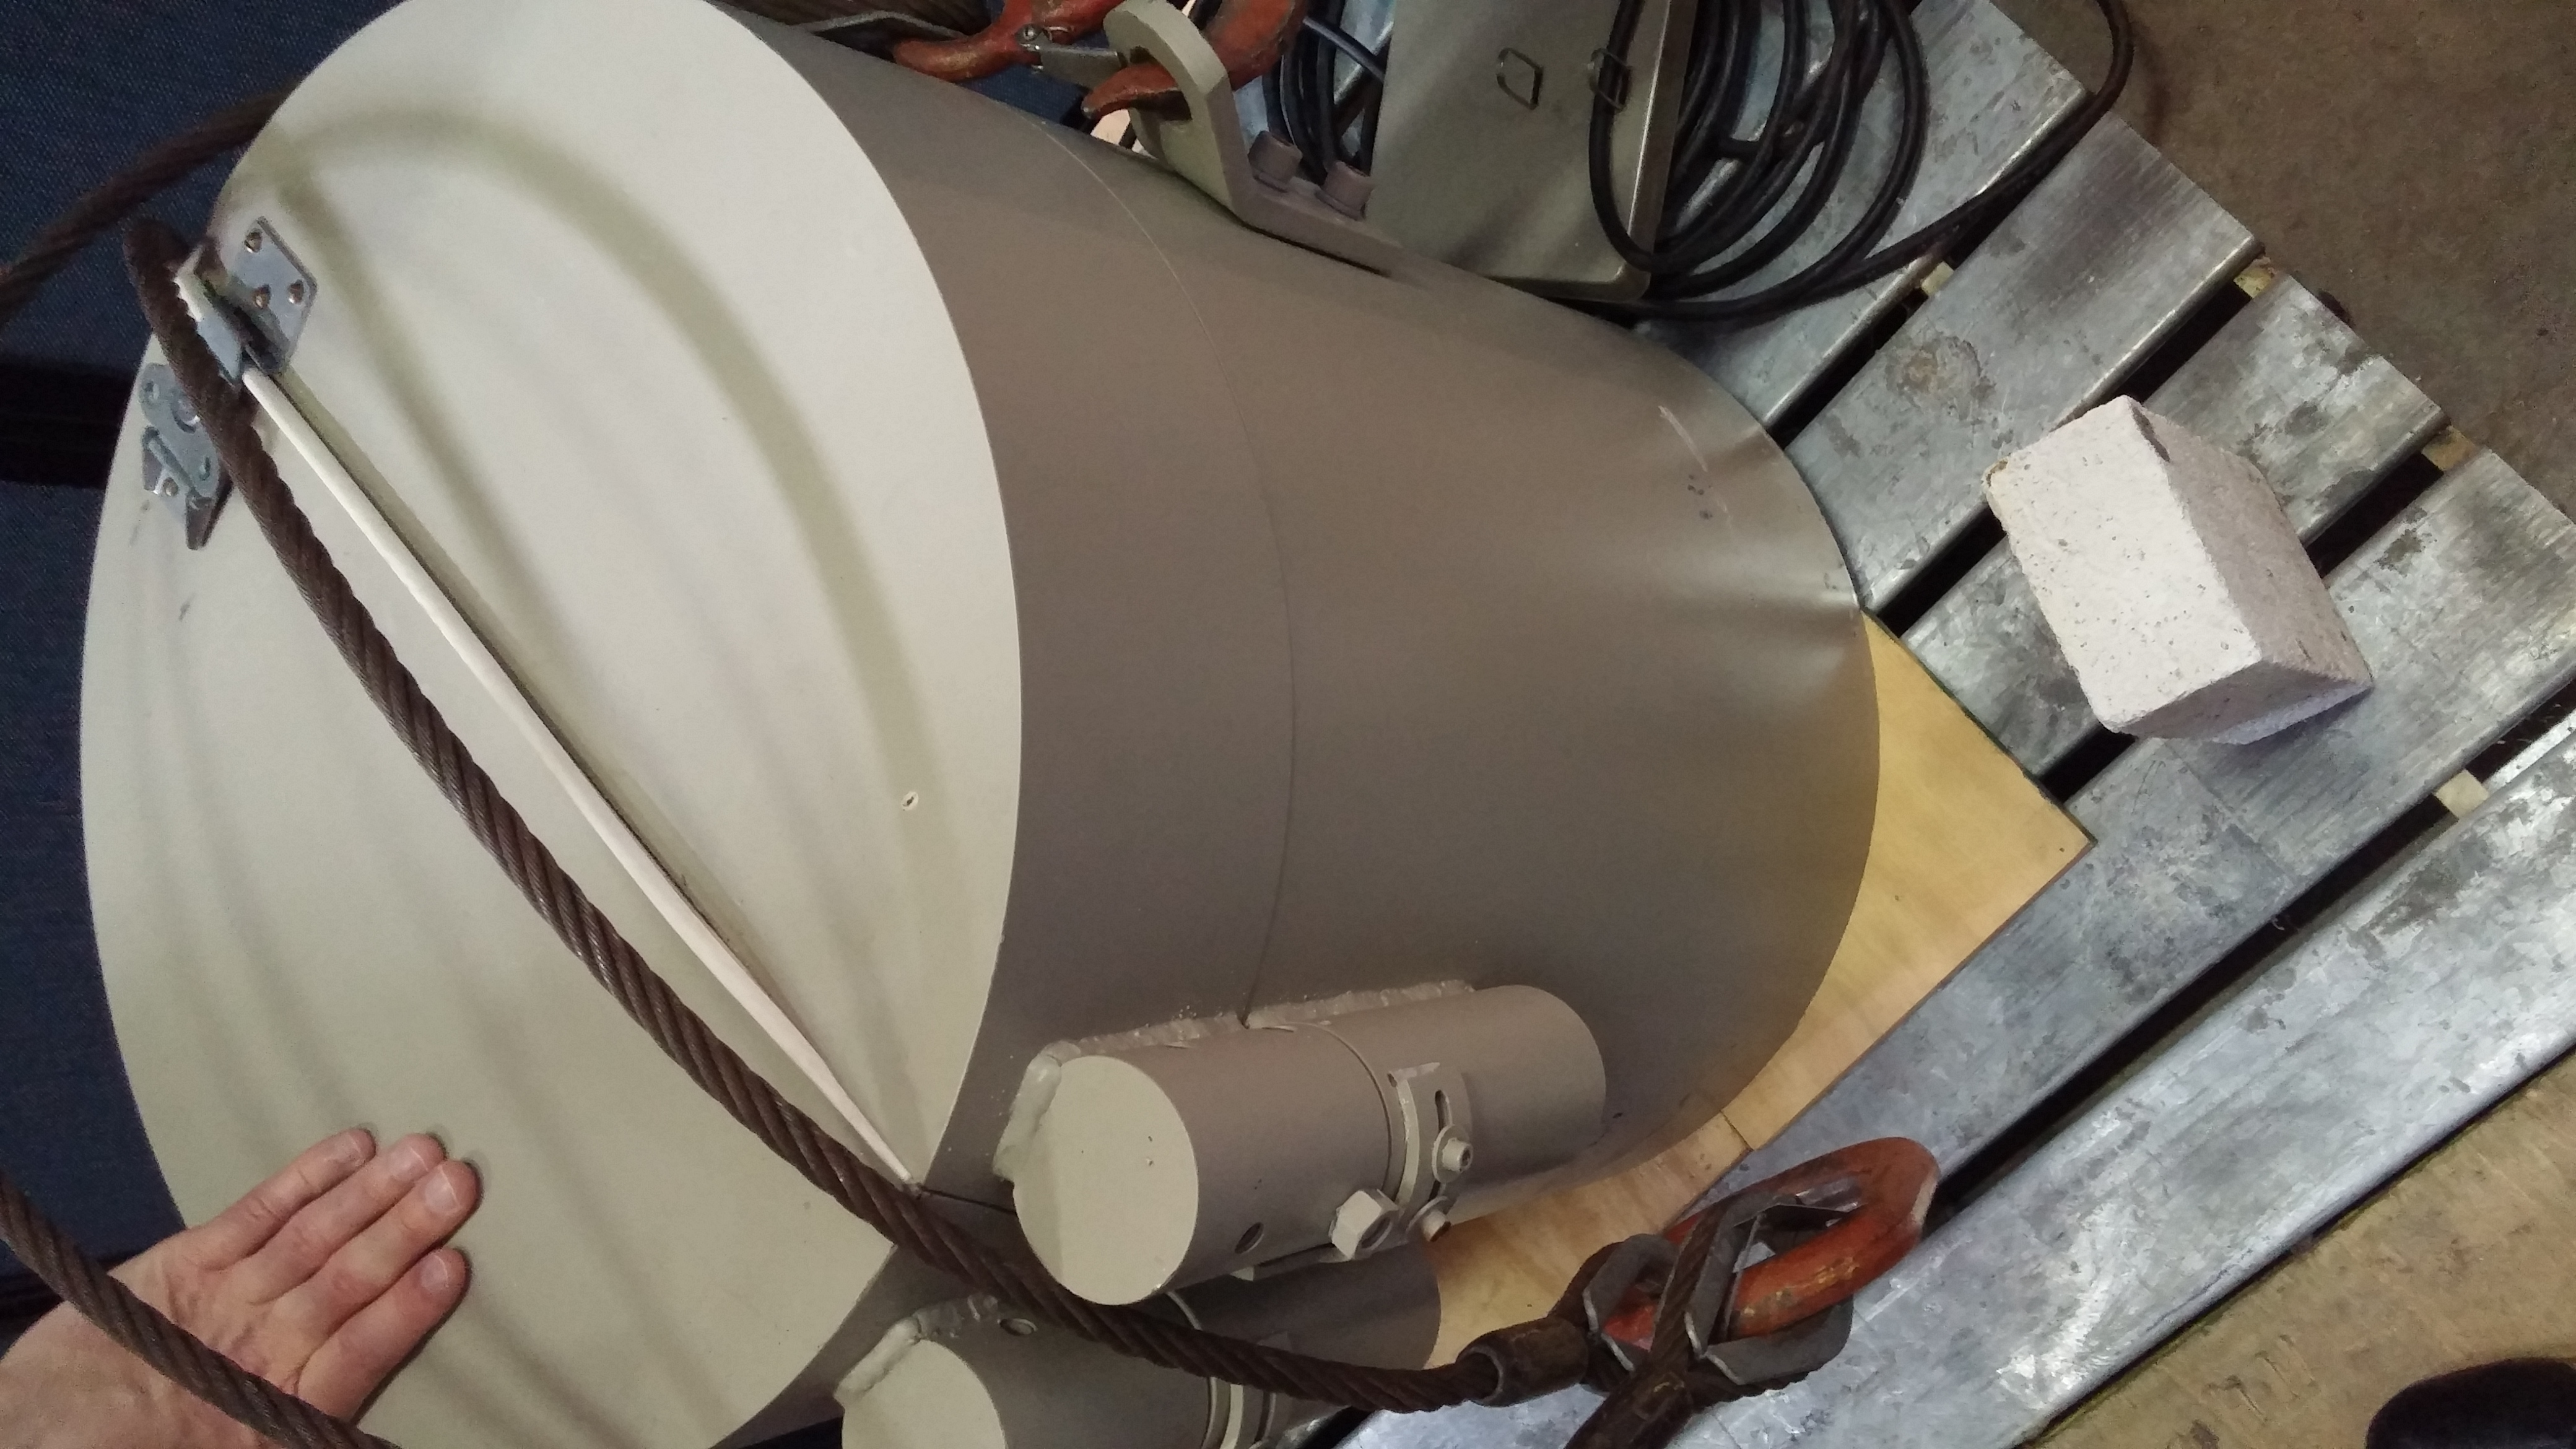
\includegraphics[width=\textwidth]{shield.jpg}
  \caption{1 tonne lead shield as seen from the outside. The lid rotates off allowing direct
  access to the acrylic vessel from the top.}
\end{figure}
\begin{figure}
  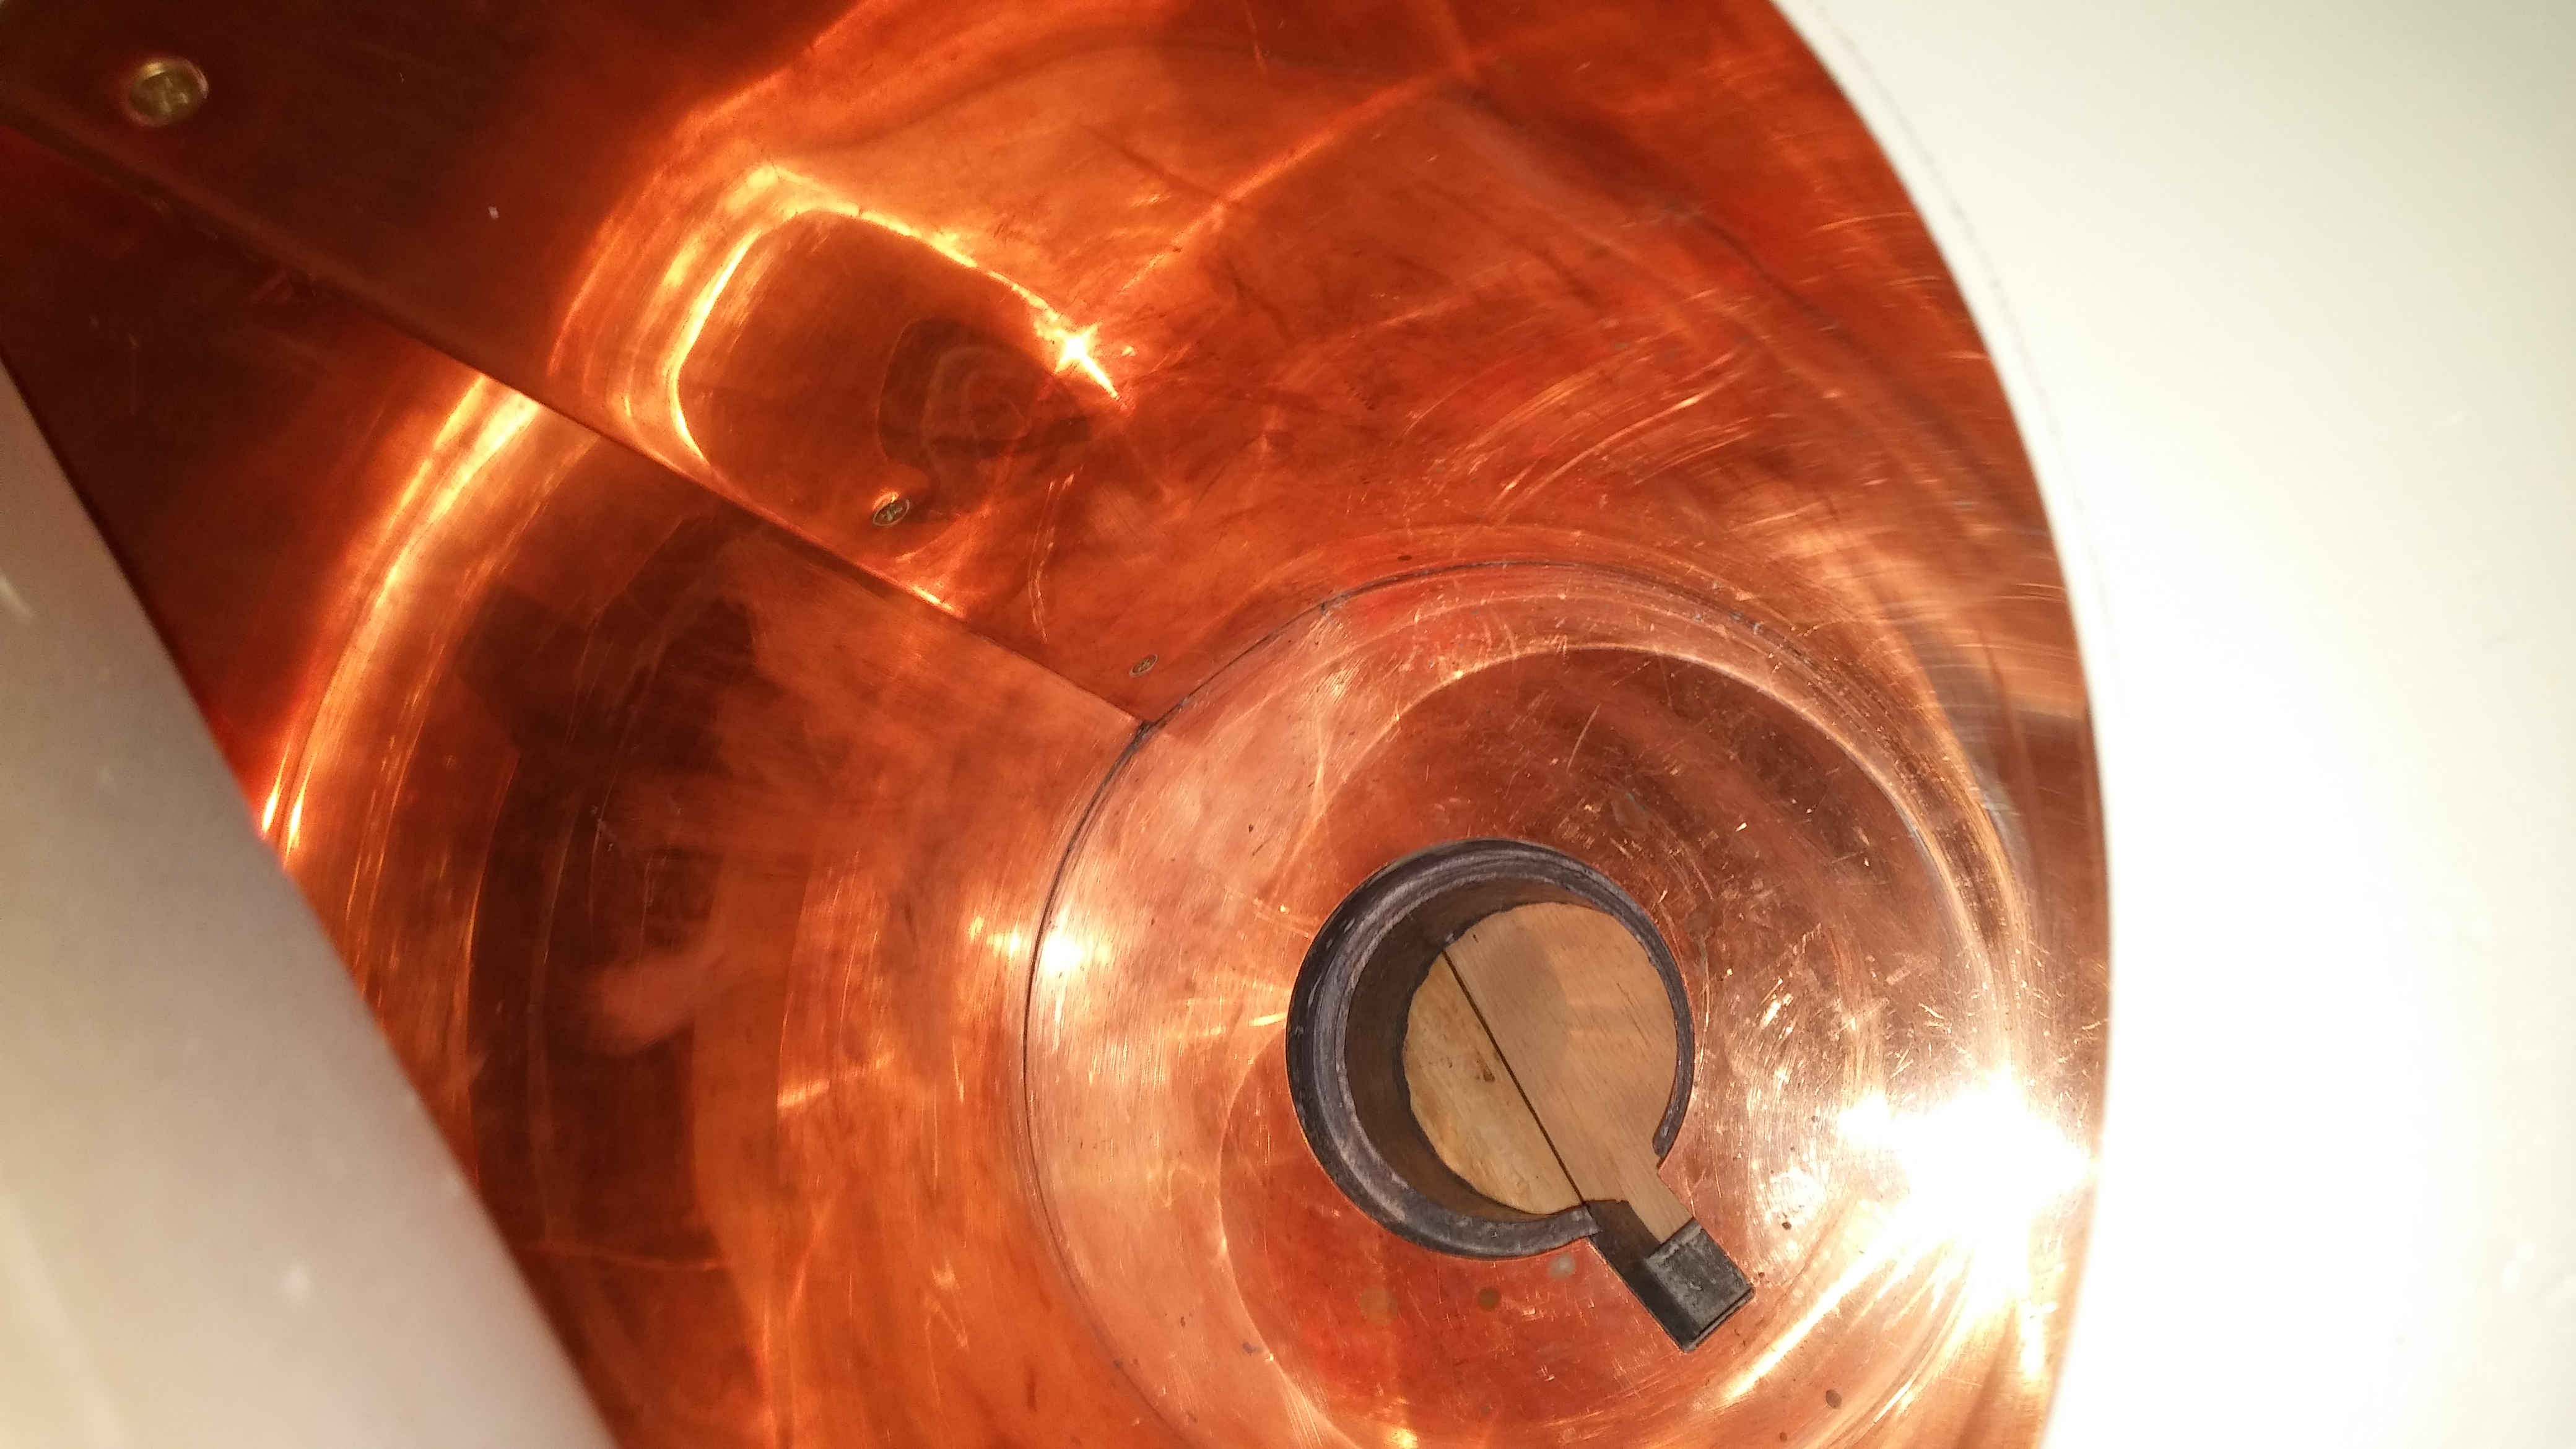
\includegraphics[width=\textwidth]{shield_inside.jpg}
  \caption{Inside of the lead shield showing the copper lining and access whole at the bottom.}
\end{figure}

\end{document}
